% !TeX spellcheck = en_GB
\documentclass[
			   fontsize=11pt,
               paper=a4,
               bibliography=totoc,
               idxtotoc,
               headsepline,
               footsepline,
               footinclude=false,
               BCOR=12mm,
               DIV=13,
               openany,   % using this removes blank pages around part / chapter starts.
%               oneside    % include this if you have to print only one page per sheet of paper.
               ]
               {scrbook}

%%% SETTINGS

% no word wrapping
%\righthyphenmin=62
%\lefthyphenmin=62
% fewer hyphens
\usepackage{microtype}

% german symbols
\usepackage[utf8]{inputenc}

% strikethrough by \sout
\usepackage[normalem]{ulem}

% insert graphics
\usepackage{graphicx}
% more flexible figures e.g. graphics with captions beside them
\usepackage{floatrow}
% more flexible captions.
% Use \captionsetup{options} to configure,
% use it in an environment for local setup
\usepackage{caption}
% subfigures (see template):
\usepackage{subcaption}

% more control of enumerations and itemizations
\usepackage{enumitem}
% less space between items
\setlist[itemize]{itemsep=0cm}
\setlist[enumerate]{itemsep=0cm}
% more customizeable tables (e.g. multiple lines per cell)
\usepackage{tabularx}
% fix for vertical centering
\usepackage{ragged2e}
\renewcommand\tabularxcolumn[1]{>{\Centering}m{#1}}
% column types with multiple lines and formatting
\usepackage{array}
\newcolumntype{C}{>{\centering\arraybackslash}X}
\newcolumntype{R}{>{\raggedleft\arraybackslash}X}
\newcolumntype{L}{>{\raggedright\arraybackslash}X}
% merge multiple rows \multirow{2}{*}{bla} & \\ &
\usepackage{multirow}
% activate for tables with page breaking
%\usepackage{ltablex}
% fix for table movement and itemizations
%\keepXColumns

% fix for dynamics spaces after custom commands
\usepackage{xspace}

% tabbing: use with \tab
\usepackage{tabto}
\TabPositions{4cm}

%% fancy math
% propper matrices, underbrace text
%\usepackage{amsmath}
\usepackage{mathtools}
% special symbols e.g. squares
\usepackage{amssymb}

%% plotting
\usepackage{pgfplots}
\usepgfplotslibrary{fillbetween}

%%Settings for code
% code placement right there
\usepackage{float}
% code coloring
\usepackage{xcolor}
% code listing
\usepackage{listings}

% flexible multi column style
\usepackage{multicol}

% graphs
\usepackage{tikz}
\usetikzlibrary{shapes.geometric, arrows}
% define some elements
\tikzstyle{box} = [rectangle, rounded corners, minimum width=3cm, minimum height=1cm,text centered, draw=black, fill=black!5]
\tikzstyle{arrow} = [thick,->,>=stealth]
\usepackage{varwidth}

% Some code highlighting styles you can use with lstlistings
% C++ code style similar to default eclipse
\lstdefinestyle{eclipse-cpp} {
    captionpos=b,
    language=C++,
    otherkeywords={final},
    basicstyle=\footnotesize,
    numbers=left,
    numberstyle=\small,
    showstringspaces=false,
    tabsize=2,
    frame=single,
    breaklines=true,
    keywordstyle=\bfseries\color[RGB]{127,0,85},
    identifierstyle=\color[RGB]{0,0,192},
    stringstyle=\color[RGB]{42,0,255},
    commentstyle=\color[RGB]{63,127,95},
}

% If no highlighting is intended
\lstdefinestyle{plain}{
	basicstyle=\ttfamily\footnotesize,
}

\lstdefinestyle{cmd}
{
	basicstyle=\ttfamily\footnotesize,
	captionpos=b,
	language=bash,
	otherkeywords={final},
	numbers=left,
	numberstyle=\small,
	showstringspaces=false,
	frame=single,
	breaklines=true,
}

% fancy algorithms (see template)
\usepackage[ruled, vlined, linesnumbered]{algorithm2e}
\DontPrintSemicolon
\SetKw{KwBy}{by}
\SetKw{KwAnd}{and}

% clickable links and clickable table of content <3
% Options: links with linebreaks
\PassOptionsToPackage{hyphens}{url}
\usepackage[bookmarks=false]{hyperref}
\hypersetup{
    colorlinks,
    citecolor=black,
    filecolor=black,
    linkcolor=black,
    urlcolor=black
}
% Alterations to labels used by \autoref{}: Capitalize everyything
\def\chapterautorefname{Chapter}
\def\sectionautorefname{Section}
\def\subsectionautorefname{Subsection}
\def\algorithmautorefname{Algorithm}
\def\subfigureautorefname{Figure}
% for custon stuff like use:
% \hyperref[custom:foo]{Custom~\ref*{custom:foo}}

% -------------------------------------------------------------------------------
% ------------------------- Bibliography Customisation ------------------------
% -------------------------------------------------------------------------------

% replace \makebibliography with this package to enable nice formatting for citing web pages
\usepackage[%
backend=bibtex				% biber or bibtex
,style=numeric-comp		% numerical-compressed TODO: Check if plain is fine as style (was 'alpha' before I changed it)
,sortcites=true				  % sorts citations if multiple entry keys are passed to a citation command
,isbn=true
,url=true
,doi=true
%,natbib=true         % if you need natbib functions
]{biblatex}
\addbibresource{literature.bib}  % better than \bibliography
\usepackage{lipsum} % for filling pages with stuff

% -------------------------------------------------------------------------------
% -------------------------- Glosssary Customisation --------------------------
% -------------------------------------------------------------------------------
% For some reason this did not work when located in settings.tex
% Any links in resulting glossary will not be "clickable" unless you load the glossaries package after the hyperref package.

\usepackage{xparse}
\usepackage[acronym,toc]{glossaries}

\DeclareDocumentCommand{\newdualentry}{O{}D<>{}m m m m m } {
	\newglossaryentry{gls-#3}{
		name={#5},
		text={#5\glsadd{gls-#3}},
		description={#6},
		plural={#7},
		#1
	}
	\newacronym[see={[Glossary:]{gls-#3}},#2]{#3}{#4}{#5\glsadd{gls-#3}}
}

% use the \newdualentry command like this:
% \newdualentry{OWD}    																			% label
% 	{OWD}		            																				 % abbreviation
% 	{One-Way Delay} 	   																				% long form
% 	{The time a packet uses through a network from one host to another}	  % description
%   {OWDs}																							   % abbreviation in plural

\newcommand{\code}[1]{\lstinline[basicstyle = \ttfamily\small]{#1}} % wrap \lstinline because texstudio doesn't parse it properly

\makeglossaries
% -------------------------------------------------------------------------------
% ---------------------- Acronyms and Glossary Definition ---------------------
% -------------------------------------------------------------------------------

\newacronym{nnapi}{NNAPI}{Neural Networks API}

\newacronym{cv}{cv}{computer vision}

\newacronym{cnn}{cnn}{convolutional neural network}

\newacronym{resnet}{ResNet}{residual neural network}

%\newacronym{relu}{ReLU}{Rectified Linear Unit}

\newacronym{ml}{ml}{machine learning}

\newacronym{ann}{ann}{artificial neural network}
	
\newdualentry{api} %oxford dictionary
	{api}
	{application programming interface}
	{set of functions and procedures allowing the creation of applications that access the features or data of an operating system, application, or other service}
	{apis}

\newglossaryentry{diff_privacy} %https://oconnell.fas.harvard.edu/files/salil/files/differential_privacy_primer_nontechnical_audience.pdf
{
	name={differential privacy},
	description={protects an individual’s information essentially as if her information were not used in the analysis at all, in the sense that the outcome of a differentially private algorithm is approximately the same whether the individual’s information was used or not}
}

% -------------------------------------------------------------------------------
% --------------------------------- Thesis Info ---------------------------------
% -------------------------------------------------------------------------------

% set title, authors and stuff for the cover
% docytype needs xspace because it is used within text.
\def\doctype{Bachelor's Thesis\xspace}

\def\studyProgram{Informatics}
\def\title{Implementing a mobile app for object detection}

\def\titleGer{Entwicklung einer mobilen App zur Objekterkennung}
\def\author{David Drews}
% Prof
\def\supervisor{Univ.-Prof. Dr. Hans-Joachim Bungartz}
% PhD Candidate
\def\advisor{Severin Reiz, M.Sc.}
\def\date{15th of August 2021}

\begin{document}
\frontmatter
% -------------------------------------------------------------------------------
% ---------------------------------- COVERPAGE ------------------------------
% -------------------------------------------------------------------------------

% correct BCOR - undo at the end !!!
\def\bcorcor{0.15cm}
\addtolength{\hoffset}{\bcorcor}
\thispagestyle{empty}
\vspace{4cm}
\begin{center}
    
\includegraphics[width=4cm]{templateStuff/tumlogo.pdf}\\[5mm]
    \huge DEPARTMENT OF INFORMATICS\\[5mm]
    \large TECHNICAL UNIVERSITY OF MUNICH\\[24mm]

    {\Large \doctype in \studyProgram}\\[20mm]
    {\huge\bf \title\par}
    \vspace{15mm}
    {\LARGE  \author}
    \vspace{10mm}
    \begin{figure}[h!]
        \centering
        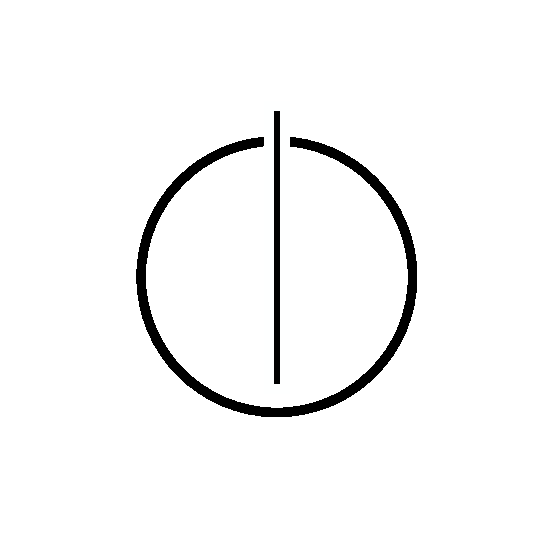
\includegraphics[width=4cm]{templateStuff/informat.pdf}
   \end{figure}
\end{center}

\cleardoubleemptypage

% -------------------------------------------------------------------------------
% ---------------------------------- TITLEPAGE --------------------------------
% -------------------------------------------------------------------------------

\def\bcorcor{0.15cm}
\addtolength{\hoffset}{\bcorcor}
\thispagestyle{empty}
\vspace{10mm}
\begin{center}
    
\includegraphics[width=4cm]{templateStuff/tumlogo.pdf}\\[5mm]
	\huge DEPARTMENT OF INFORMATICS\\[5mm]
	\large TECHNICAL UNIVERSITY OF MUNICH\\[24mm]
	{\Large \doctype in \studyProgram}\\[20mm]
	{\LARGE\textbf \title}\\[10mm]
	{\LARGE\textbf \titleGer}\\[10mm]
	\begin{tabular}{ll}
		\Large Author:      	& \Large \author \\[2mm]
		\Large Supervisor:  	& \Large \supervisor\\[2mm]
		\Large Advisor:			& \Large \advisor\\[2mm]
		\Large Submission Date:       		& \Large \date
	\end{tabular}
	\vspace{-1mm}
	\begin{figure}[h!]
		\centering
		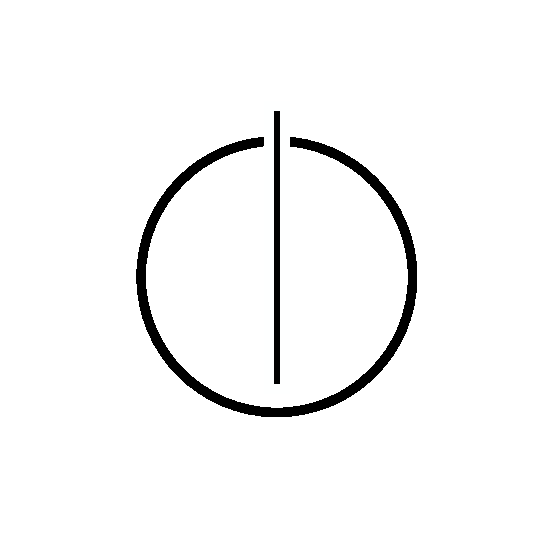
\includegraphics[width=4cm]{templateStuff/informat.pdf}
	\end{figure}
\end{center}

% undo BCOR correction
\addtolength{\hoffset}{\bcorcor}
\newpage

% -------------------------------------------------------------------------------
% ---------------------------------- DISCLAIMER -------------------------------
% -------------------------------------------------------------------------------

\cleardoubleemptypage

\thispagestyle{empty}
\vspace*{0.7\textheight}
\noindent
I confirm that this \MakeLowercase{\doctype} is my own work and I have documented all sources and material used.\\

\vspace{15mm}
\noindent
Munich, \date \hspace{5cm} \author
\cleardoubleemptypage

% -------------------------------------------------------------------------------
% ---------------------------------- ABSTRACT --------------------------------
% -------------------------------------------------------------------------------

\phantomsection
\addcontentsline{toc}{chapter}{Abstract}
\vspace*{2cm}
\begin{center}
    {\Large \textbf {Abstract}}
\end{center}
\vspace{1cm}

We migrate the entire code base of the Android application TUM-Lens from Java to Kotlin. This facilitates the future development of the app as it makes the code more concise and error-proof. Consequently, we elaborate on further advantages of the Kotlin language over Java and analyse how this migration lowered the lines of the existing code. Moreover, we expand the functionalities of the app by an object detection feature based on Google's open source deep learning framework TensorFlow Lite. The implementation follows in the previous TUM-Lens developer's footsteps and integrates the object detection to entirely work on-device so that no data needs to be exchanged with external servers. On the object detection theory side, we distinguish object detection from other visual machine learning tasks and survey a selection of modern deep learning architectures - both for backbone and detector networks. In addition, we study the mechanics of a specific model in detail, the SSD MobileNet v1, as this is the model applied to the object detection task in TUM-Lens. This thesis expands Maximilian Jokel's previous work \textit{Implementing a TensorFlow-Slim based Android app for image classification} (2020).

\cleardoublepage

% -------------------------------------------------------------------------------
% ------------------------------ TABLE OF CONTENTS -------------------------
% -------------------------------------------------------------------------------

\tableofcontents
\thispagestyle{empty}
\cleardoubleemptypage

% -------------------------------------------------------------------------------
% --------------------------------- MAIN MATTER ------------------------------
% -------------------------------------------------------------------------------

\mainmatter

\chapter{Motivation}

The aim of this work was to further develop the Android app TUM-Lens \cite{lensApp}. Its core function is the analysis of images that are captured by the camera of the Android device and transmitted to the app as a live feed. With the completion of this work, the pre-existing image classification capabilities of the app are now complemented with object detection.

For an optimal user experience, the analysis of the images must take place in near real time. This is the only way to ensure that the analysis results displayed always match the current content of the camera feed, which can change very quickly due to panning of the camera by its user. While in many applications the analysis of image data can take place decentrally in powerful data centres, in the case of TUM-Lens the image analysis runs on the mobile device itself.

%\section{Increasing Computation Power on Mobile Devices} %TODO: will probably not elaborate here as 3 topics for motivation might be enough

\section{Growing Support for On-Device Machine Learning}

Support for the development of \gls{ml} and also in particular deep learning applications for mobile platforms is growing steadily and from different directions at the same time. Developer-friendly frameworks such as TensorFlow\footnote{\url{https://www.tensorflow.org/}}, developed by Google Brain, or PyTorch\footnote{\url{https://pytorch.org/}}, developed by Facebook's AI Research Lab, are among the best-known deep learning frameworks~\cite{dl_ranking_2018}. The releases of TensorFlow Lite\footnote{\url{https://www.tensorflow.org/lite}} 2017~\cite{tflite_release_verge_2017} and PyTorch Mobile\footnote{\url{https://pytorch.org/mobile/home/}} 2019~\cite{pytorch_release_2019} show that mobile platforms increasingly come into focus of companies providing \acrlong{ml} software. In recent years, device manufacturers and operating system developers also started to provide dedicated hardware and software components for mobile machine learning. Examples include Apple's Neural Engine~\cite{neural_engine_verge_2017}, unveiled in 2017, or Android's \gls{nnapi}~\cite{nnapi_devguide_2021}. Apple's Neural Engine is a hardware component optimised for \acrlong{ml} requirements. Android's \gls{nnapi}, on the other hand, is an Android C \gls{api} for efficient computation of \gls{ml} operations and provides a basic set of functions for higher-level \gls{ml} frameworks. As a result of these developments, it is becoming easier for developers to build \gls{ml} applications that run efficiently on mobile devices. This support was a major catalyst for the initial and further development of TUM-Lens in the context of two bachelor theses.

\section{Offline Usability}

TUM-Lens is more independent compared to many other \acrlong{ml} based apps as it does not require an internet connection to use it. Often, apps and services require a connection to the internet because of the nature of the task they are meant to perform. The Amazon voice assistant Alexa can answer simple voice commands to control smart home devices or check the time without having access to the world wide web and thus already uses on-device \acrlong{ml}. But even if Alexa could analyse and understand all voice commands locally, the request would still have to be forwarded to the Amazon servers in most cases. Due to the large number of possible queries, not all answers can be kept on the device, but must be retrieved from a data centre that has more storage capacity. Such queries include daily topics such as the weather report, traffic or the result of a sporting event. However, an internet connection is not required to use the full range of functions of TUM-Lens. All the information needed for image classification and object detection is stored locally on the device in the form of various already trained \gls{ann}. With the integration of the corresponding mobile frameworks, the image analysis can therefore be carried out locally on the device, making the app independent of an internet connection.

\section{Improved Privacy}

The use of on-device \gls{ml} provides a further mechanism for protecting personal data in the context of machine learning in addition to existing methods such as \gls{diff_privacy}. Due to the growing support for mobile \gls{ml} applications mentioned above, but also due to the continually increasing power of mobile devices~\cite{mobile_cpu_power}, not only the use of pre-trained \glspl{ann} becomes possible, but also the training of new \glspl{ann} on the mobile device itself becomes more and more feasible and relevant~\cite{liu19}. If the training process takes place locally on the device itself, no data needs to be transferred to external instances such as a company's servers. This makes it possible to develop applications that adapt more and more individually to the user as they are used, while guaranteeing a maximum level of data protection. An example of the development of such an application is DeepType~\cite{deepType}. DeepType attempts to predict the next word used when the user enters the keyboard. While every user initially starts with the same pre-trained version of the \gls{ann} used by DeepType, the application continues to train this \gls{ann} with each input and thus adapts more and more to the characteristic input behaviour of the user - all without the text inputs ever leaving the device.


\chapter{Important Concepts}

Everyone is talking about machine learning. It is already impossible to imagine our everyday life without the use of the term. Due to the multitude of contexts in which machine learning is spoken of, some justifiably and some unjustifiably, it is important to create a common understanding of some machine learning-related concepts in order to ensure a common understanding of the theoretical contents of this work.

%TODO: Maybe outline the different concepts that will be explained as their connection is loser than the other parts of the thesis.

\section{Machine Learning}

A popular definition of \gls{ml} is attributed to Arthur Samuel describing it as the "field of study that gives computers the ability to learn without being explicitly programmed"\footnote{Althought cited in popular machine learning material like Andrew Ng's \gls{ml} course at Stanford~\cite{mlCourseStan} the quote appears neither in Samuel's 1959~\cite{mlQuote1959} nor his 1967 paper~\cite{mlQuote1967}.}. \acrlong{ml} algorithms circumvent this need for explicit programming by improving an internal model through data. This process is called training and the data used to train the model is often regarded to as the model's experience~\cite{mlMitchell}. As depicted in figure \autoref{fig:mlClassification}, \gls{ml} can be divided into the subfields supervised learning, unsupervised learning, semi-supervised learning and reinforcement learning.

\begin{figure}[H]
	\centering
	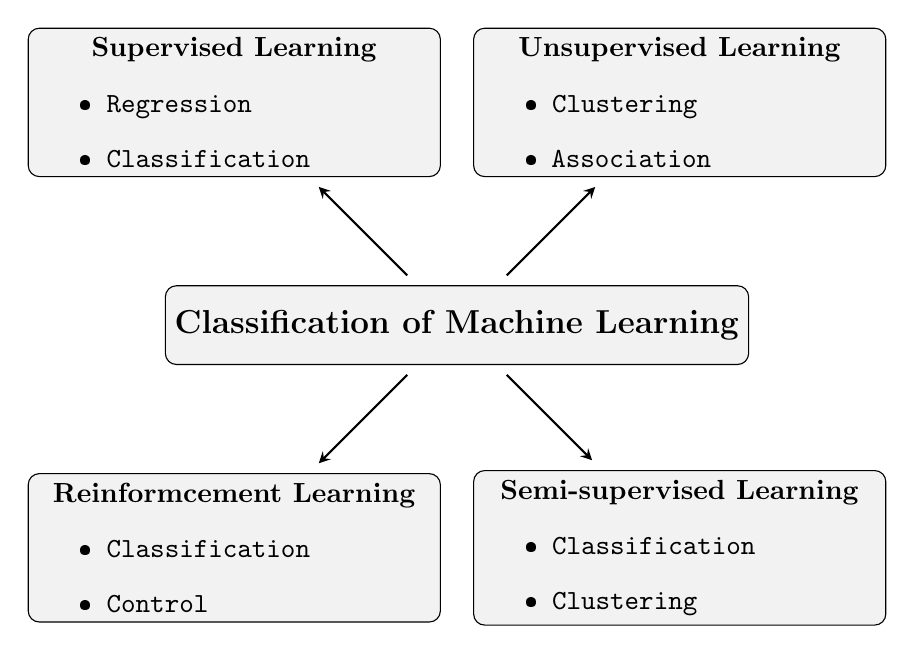
\begin{tikzpicture}[node distance=4cm]
		\node[box] (ml) {\large{\textbf{Classification of Machine Learning}}};
		\node[box, above left of = ml] (supervised) {
			\begin{minipage}{5cm}
				\centering\textbf{Supervised Learning}
				\begin{itemize}
					\item \texttt{Regression}
					\item \texttt{Classification}
				\end{itemize}
			\end{minipage}
		};
		\node[box, above right of = ml] (unsupervised) {
			\begin{minipage}{5cm}
				\centering\textbf{Unsupervised Learning}
				\begin{itemize}
					\item \texttt{Clustering}
					\item \texttt{Association}
				\end{itemize}
			\end{minipage}
		};
		\node[box,  below right of = ml] (semisupervised) {
			\begin{minipage}{5cm}
				\centering\textbf{Semi-supervised Learning}
				\begin{itemize}
					\item \texttt{Classification}
					\item \texttt{Clustering}
				\end{itemize}
			\end{minipage}
		};

		\node[box, below left of = ml] (reinforcement) {
			\begin{minipage}{5cm}
				\centering\textbf{Reinformcement Learning}
				\begin{itemize}
					\item \texttt{Classification}
					\item \texttt{Control}
				\end{itemize}
			\end{minipage}
		};
		\draw[arrow, shorten >= 5pt, shorten <= 5pt] (ml) -- (supervised);
		\draw[arrow, shorten >= 5pt, shorten <= 5pt] (ml) -- (unsupervised);
		\draw[arrow, shorten >= 5pt, shorten <= 5pt] (ml) -- (semisupervised);
		\draw[arrow, shorten >= 5pt, shorten <= 5pt] (ml) -- (reinforcement);
	\end{tikzpicture}
	\caption[Classification of Machine Learning]{The field of \acrlong{ml} divided into subfields by the characteristics of the underlying learning process. Also indicates the learning problems that are typically tried to be solved by applying the respective learning process.}
	\label{fig:mlClassification}
\end{figure}

\subsection{Supervised Learning}
In supervised learning, the learning machine is provided with input data as well as the output that is expected for the given input~\cite{introSupervised}. In the classical case of spam filtering, the input can be a collection of emails and the expected output is a label attached to each email that either classifies it as spam or as non-spam. The learning machine is then fed all e-mails as input data and learns to recognise which information in the input is important to produce the correct classification. As the system knows the correct answer for each training input, it can process an email, predict whether or not it is spam, and then use the known answer to change its weights in a way that will make it more likely to lead to a correct prediction and less likely to lead to a false prediction the next time it is presented with similar input.

\subsection{Unsupervised Learning}
Detecting hidden patterns and structuring data is where unsupervised learning comes into play. Learners of this type don't need to be provided with an expected output while being trained~\cite{introUnsupervised}. A scenario for the application of unsupervised learning is the problem of dividing a customer base into subgroups in order to treat every subgroup according to their specific needs. An employee might help the machine learning system by providing the number of subgroups she wants the system to generate. The learner then builds up its representation of the internal structure of the entire data set with every input it processes. After having processed enough customers, it will most likely have identified the key metrics that distinguish customers into the different groups. 

\subsection{Semi-Supervised Learning}
One use for semi-supervised learning is cluster analysis, which was already used as an example in the previous paragraph. In the case of semi-supervised learning, the system no longer has to work out the different groups (also known as \textit{clusters}) from the unlabelled data alone. Instead, it can use a small set of already labelled customers as a reference and build its internal representation of the entire dataset (labelled and unlabelled) around the clusters indicated by the pre-labelled data. This is especially useful because in many domains collecting or creating labelled data is difficult, expensive, or both~\cite{introSemiSup}.

\subsection{Reinforcement Learning}

Reinforcement learning is "learning what to do - how to map situations to actions - so as to maximize a numerical reward signal"~\cite{introRL}. Systems are trained via reinforcement learning to learn how to behave in dynamic environments. The tasks in these environments can stretch from playing a video game~\cite{rlStarCraft} to driving an autonomous car~\cite{rlCars}. These exemplary tasks show two characteristics that distinguish reinforcement learning from the other subfields of \gls{ml}: The reward signal is often delayed and attribution to single actions is difficult. Only once a game is won or the car has arrived safely at its destination the system knows if all the decisions it made along the way lead to a positive outcome. \textit{Trial-and-error} is therefore a term that summarises this learning paradigm quite precisely.


\section{Artificial Neural Networks} \label{ssection:ann}

An \acrlong{ann} - often just referred to as neural network - is a data processing concept that is inspired by biological neurons and their interconnectivity. As figures \autoref{fig:2layeredANN} and \autoref{fig:3layeredANN} show the artificial neurons (also called \textit{nodes}) in an \gls{ann} are grouped in \textit{layers}. There are three important types of layers: The \textit{input layer}\footnote{Note that the input layer is not counted towards the total number of layers in an \gls{ann}.}, the \textit{output layer} and an arbitrary number of \textit{hidden layers} in between the input and output layer. Similar to neurons in human brains, nodes of different layers can be connected. In \glspl{ann}, the nodes exchange signals in the form of numbers. Each node outputs a number that is computed by applying a non-linear function to its inputs. The output signal can then be a new input for other nodes or it can be part of the result returned by the output layer. The connections between nodes are also known as \textit{edges} and typically carry a weight. In the case of \glspl{ann}, the training process that is typical for all machine learning systems is the adjustment of these connection weights. The weights and other variables of the \gls{ann} are grouped under the term \textit{parameters}. In summary, an \gls{ann} transforms an input vector into an output vector through a series of non-linear functions, where both the calculation of the output and the training process are characterised by the specific structure of the \gls{ann} and its parameters.

%TODO: Maybe introduce a view typical ANN architectures like feed forward, convolutional, recurring, etc.

\section{Deep Learning}

Deep learning is a subarea of machine learning. Deep learning is characterised by the use of \glspl{ann} with many hidden layers. The more hidden layers a network has, the deeper it is. The deeper a network is and the more nodes the network has per layer, the more complex the computations that the \gls{ann} can successfully perform~\cite{dlBookGoodf}. As the number of layers and nodes grows, so does the number of parameters. Their large number is the reason deep learning requires extensive amounts of data to provide adequate results compared to other sub-disciplines of machine learning. Networks of this genus have been given the ability to perform extraordinarily complex computations at the expense of a resource-intensive training process.

\begin{multicols}{2} % defines an environment with two columns
	\begin{figure}[H] % [H] for EXACTLY HERE
		\centering
		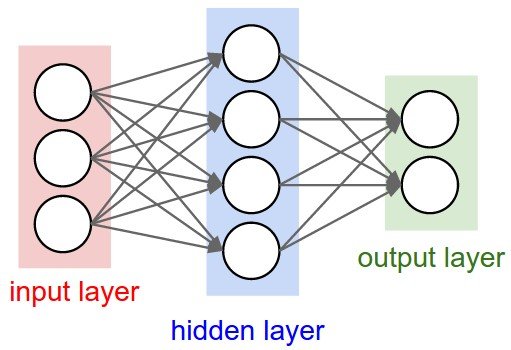
\includegraphics[height=3cm]{figures/ann1.jpeg}
		\caption[2-Layered ANN]{2-layered \gls{ann}. It is called fully connected as every node from the previous layer is connected to every node in the next layer. \\
			\tiny{Source:~\cite{annGraphics}}}
		\label{fig:2layeredANN} % labels always have to be placed after the caption
	\end{figure}
	
	\columnbreak    % start next column
	
	\begin{figure}[H] % [H] for EXACTLY HERE
		\centering
		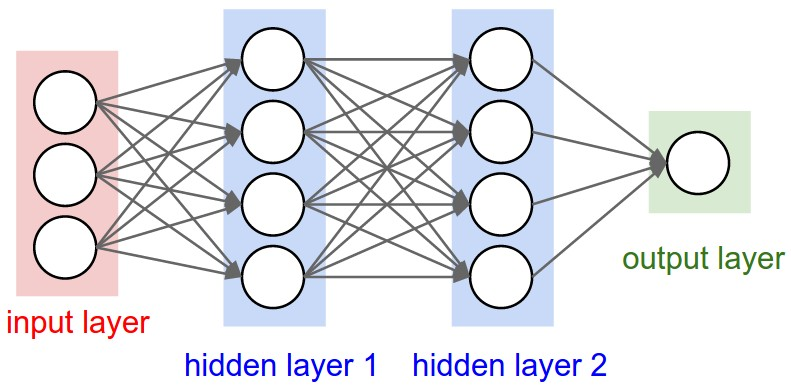
\includegraphics[height=3cm]{figures/ann2.jpeg}
		\caption[3-Layered ANN]{3-layered \gls{ann}. In \glspl{ann}, nodes in one layer are connected to nodes in other layers but not to other nodes in the same layer. \\
			\tiny{Source:~\cite{annGraphics}}}
		\label{fig:3layeredANN} % labels always have to be placed after the caption
	\end{figure}
\end{multicols}

\chapter{Object Detection}

\section{How Object Detection Differs From Related Tasks} \label{sec:cvtasks}

The field of \gls{cv} encompasses numerous distinct problems and an even larger number of potential solutions. In the following, object detection as a typical task in the \gls{cv} context is distinguished from other \gls{cv} tasks that are closest to it in terms of learning objectives.

\begin{figure}[H] % [H] for HERE
	\centering
	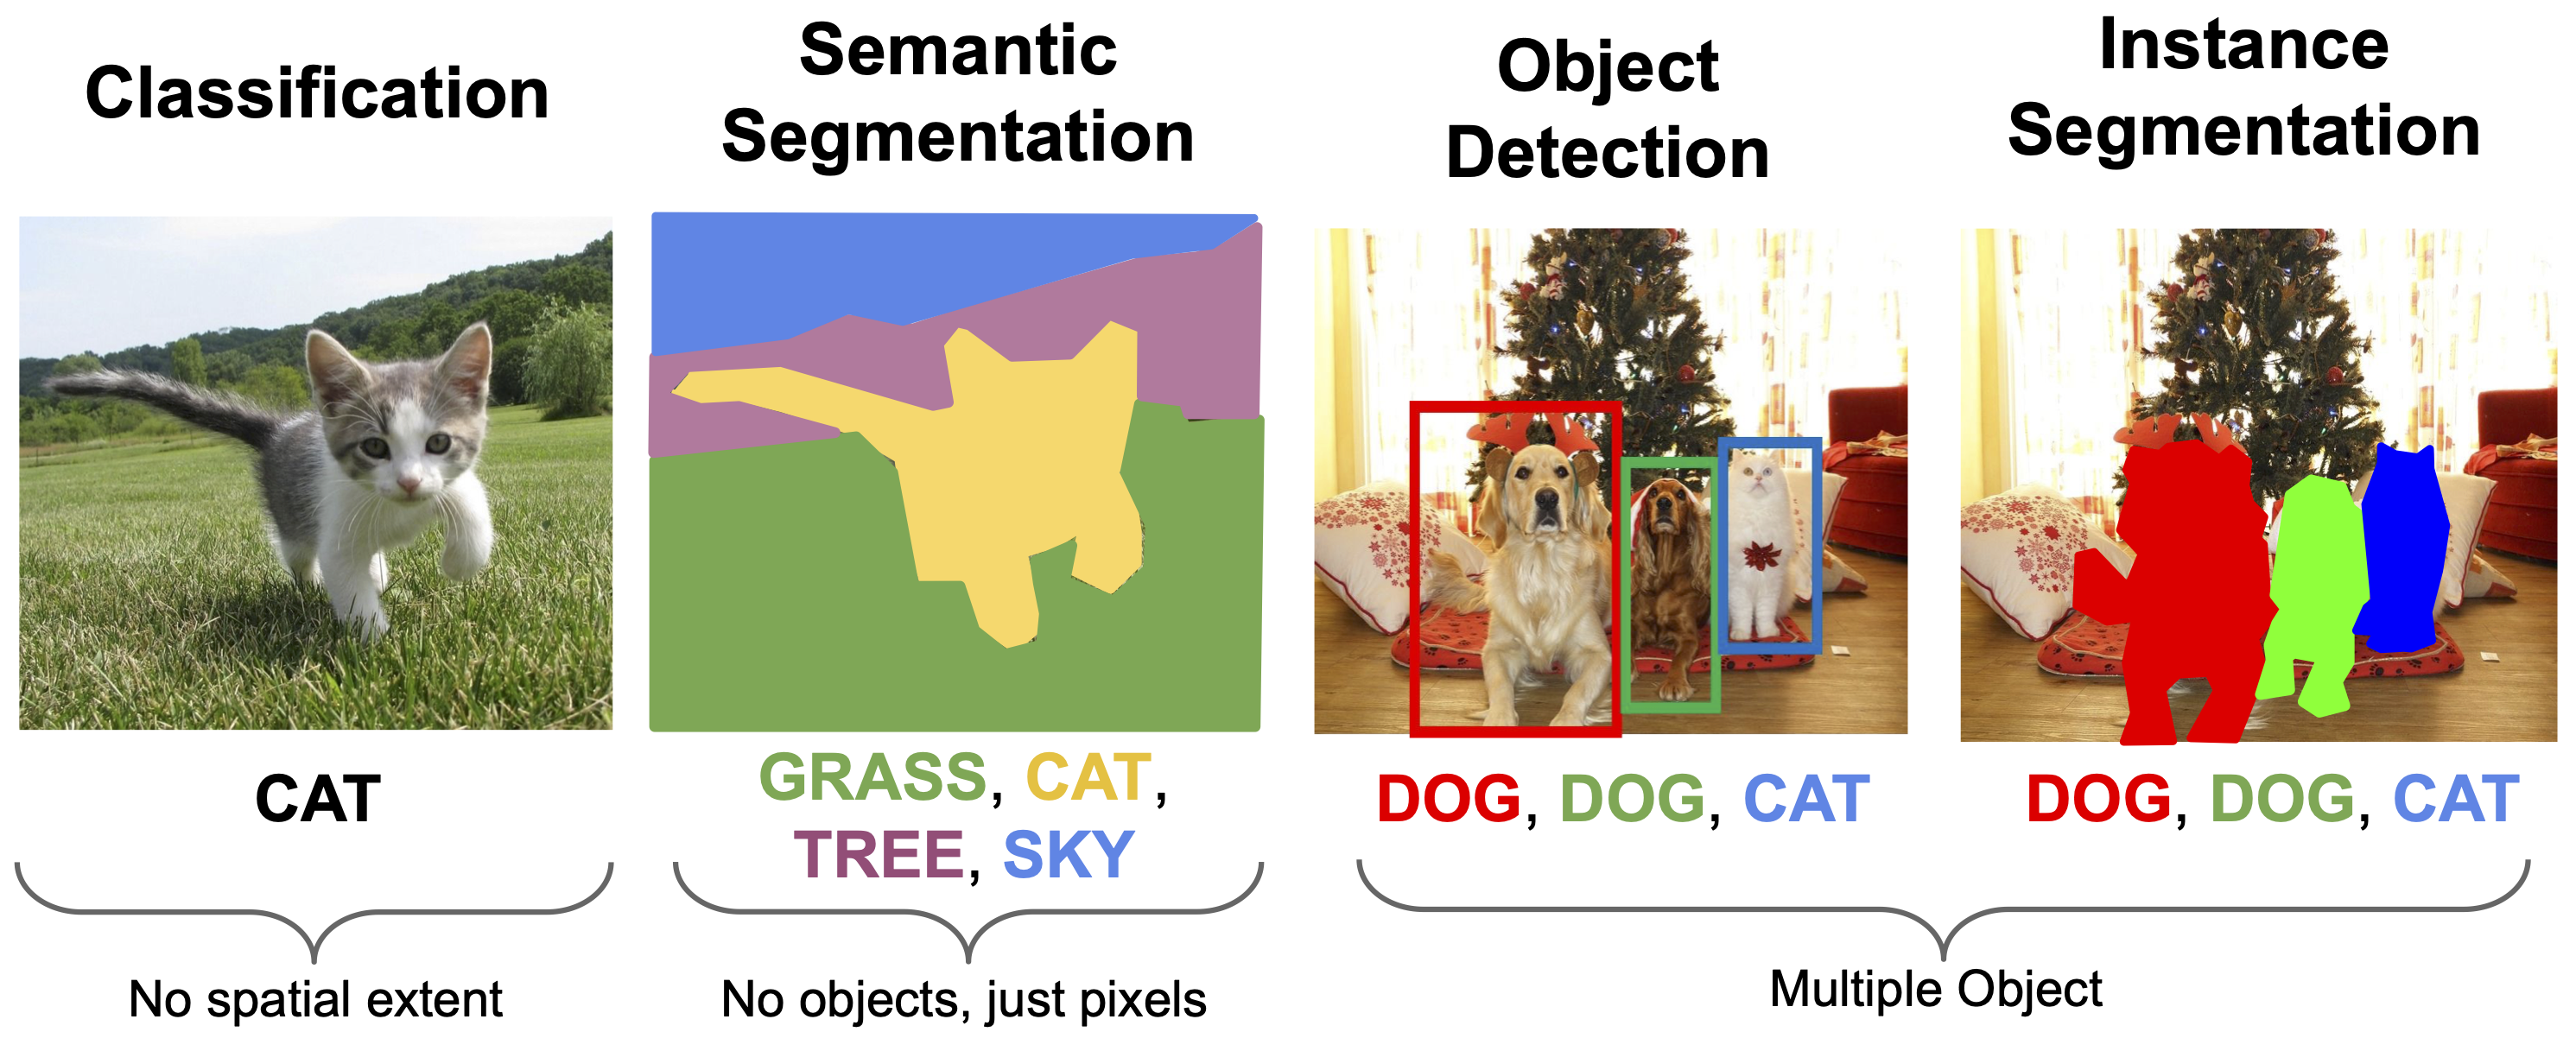
\includegraphics[width=\textwidth]{figures/detection_related_tasks.png}
	\caption[Typical Computer Vision Tasks]{Object detection differs conceptually from other related \gls{cv} tasks regarding spatial information, the concept of objects and the number of detections in a scene.\\
		\tiny{Source:~\cite{cvTasks}}}
	\label{fig:cvTasks} % labels always have to be placed after the caption
\end{figure}

\subsection{Semantic Segmentation}
In semantic segmentation, each pixel of an image is assigned a class. However, there are no objects. This means that if there are several objects of the same class in the image, all the associated pixels receive the same class label. Therefore, the different objects cannot be differentiated based on the result of the semantic segmentation.

\subsection{Image Classification}
In image classification, the result of the detection is a single class. In rare application variants, a bounding box for one object of the detected class is also returned - as a rule, however, no spatial extent is associated with the task of classification.

\subsection{Object Detection}
Object detection deals with the identification of any number of objects within an image. For each object, a class label and its position are returned as the coordinates of a rectangle enclosing the object. It is important here that, as depicted in Figure \autoref{fig:cvTasks}, several objects of the same class can also be recognised. In contrast to the  task of semantic segmentation, the different objects of the same class can be distinguished.

\subsection{Instance Segmentation}
The instance segmentation essentially fulfils a better variant of the object detection. Again, several objects of different classes are detected and the positions of the classes are also part of the output. However, the positions are not marked by bounding boxes as in object detection, but each pixel belonging to an object receives a label of this object. The objects are therefore even more sharply separated from the image areas that do not contain an object and, in contrast to semantic segmentation, individual objects of the same class remain distinguishable.

%\section{Computer Vision on Mobile Devices}

\section{Object Detection Frameworks}

State of the art object detection frameworks run predominantly on deep learning architectures~\cite{dlForDetection}. The bachelor's thesis preceding this work, \textit{Implementing a TensorFlow-Slim based Android app for image classification}~\cite{maxJokel}, already explains how \glspl{cnn} work and why they are the most important building blocks for deep learning frameworks solving perceptual tasks. This explanation will therefore not be pursued here once more. Instead, we survey a range of modern object detection frameworks. Each framework is defined by the combination of a backbone and a detector. The selection was not put together at random but is based on popularity and performance in standard object detection benchmarks~\cite{backbones}. %TODO: add reference for detection frameworks

\subsection{Backbones} \label{ssec:backbones}

The term \textit{backbone} in the context of \glspl{ann} might be used differently depending on the task pursued. In the case of visual tasks and this thesis, the backbone is the part of an object detection framework that extracts features from the input data. This encapsulation of the feature extraction task in its own set of \glspl{cnn} allows the designer of the object detection pipeline to swap and test different backbones for the task at hand~\cite{backbones}.

\begin{table}[H]
	\begin{tabularx}{\columnwidth}{C | C | C}
		\hline
		backbone					& first publication & detectors \\
		\hline \hline
		AlexNet						  & 2012 \cite{backboneAlexNet}			& HyperNet \cite{detectorHyperNet} \\
		\hline
		VGG-16						 & 2014 \cite{backboneVGG}			   & PFPNet-R512 [K] \\
		\hline
		GoogLeNet			   	   & 2014 \cite{backboneGoogLeNet}			 & YOLOv1 \cite{detectorYOLOv1} \\
		\hline
		ResNets					  	  & 2015 \cite{backboneResNet}		   & BlitzNet512 \cite{detectorBlitzNet}, CoupleNet \cite{detectorCoupleNet}, RetinaNet \cite{detectorRetinaNet},  Faster R-CNN [A], R-FCN ? \\
		\hline
		Inception-ResNet-V2   & tbd					  & Faster R-CNN G-RMI [23], Faster R-CNN with TDM [24] \\
		\hline
		DarkNet-19					& tbd					& YOLOv2 [J] \\
		\hline
		MobileNet					 & 2017 \cite{backboneMobileNet}					 & SSDv2 \\		
	\end{tabularx}
	\caption[Modern CNN Backbones and Detectors]{Overview of modern \gls{cnn} backbone networks and detectors that build upon them.}
	\label{tab:backbonesDetectors}
\end{table}

TO-DO: further sources: \\
 https://scholar.google.com/scholar?q=Dai%2C%20J.%2C%20Li%2C%20Y.%2C%20He%2C%20K.%2C%20Sun%2C%20J.%3A%20R-FCN%3A%20object%20detection%20via%20region-based%20fully%20convolutional%20networks.%20In%3A%20Lee%2C%20D.D.%2C%20Sugiyama%2C%20M.%2C%20Luxburg%2C%20U.V.%2C%20Guyon%2C%20I.%2C%20Garnett%2C%20R.%20%28eds.%29%20Advances%20in%20Neural%20Information%20Processing%20Systems%2029%2C%20pp.%20379%E2%80%93387.%20Curran%20Associates%2C%20Inc.%20%282016%29
J: http://arxiv.org/abs/1612.08242
%K: https://doi.org/10.1007/978-3-030-01228-1_15

\subsubsection{AlexNet}



\subsubsection{ResNet}

While the baseline \gls{ann} described in \autoref{ssection:ann} only connects adjacent layers, \glspl{resnet} are a special subclass of \gls{ann} that introduces \textit{shortcut connections}~\cite{backboneResNet}. Shortcut connection are edges in the network that skip one or more layers.

\subsubsection{MobileNet}
As the name suggests, MobileNets were developed especially for mobile or embedded computer vision applications. The key innovation of the MobileNet architecture is the combination of two elements:
\begin{enumerate}
	\item utilisation of depth-wise separable filters~\cite{depthSep}
	\item a network structure that enables the developer to scale the model size down by adjusting only two hyper-parameters
\end{enumerate}
As a MobileNet is a building block of the detection framework implemented in TUM-Lens, a more detailed description can be found in \autoref{ssec:mobilenetArchitecture}.


\subsection{Two-Stage Detectors}

This class of detectors separates the object detection task into two distinct stages~\cite{12stageSYNASC2018}. The network of the first stage (named Region Proposal Network (RPN) in the context of the R-CNN detector family) uses the image data to generate region proposals. The second stage is a separate network that takes these region proposals (or ROI - short for regions of interest), potentially decreases the final number of ROI using mechanics that depend on the specific detector, and then performs the classification on each of the final regions. The classified regions are then returned as the detected objects. Two-stage detectors tend to have a higher localization and object recognition accuracy than single-stage detectors but can only achieve that at the cost of considerably slower inference speed~\cite{surveyICBDT2019}. Table \autoref{tab:backbonesDetectors} shows a selection of popular detectors including R-CNN and some of its many successors, Fast-CNN and Faster-CNN.
%TODO make sure they really do appear in the tabel



\subsection{R-CNN}

R-CNN was 
Fast, Faster R-CNN, and other advancements like Mask-R-CNN
2014 \cite{detectorRCNN}

\subsection{Single-Stage Detectors}

Detection frameworks are considered to have only a single stage when they consist of one deep neural network only and compute the objects (bounding box coordinates and category) in a single pass through that network. By eliminating the explicit generation of region proposals, single-stage detectors outperform their two-stage competitors with respect to speed while sacrificing a bit of detection accuracy, if at all~\cite{detectorSSD}. %TODO: Cite more sources
This speed improvement makes single-stage detectors the preferred choice for applications running on mobile or embedded devices or in applications that require real-time image detection. Since the object detector implemented in TUM-Lens is described thoroughly in \autoref{sec:mobilessd}, the following overview of selected single-state detectors will help us to understand how the app's object detector differs from other possible options.

\subsubsection{RetinaNet}

2018

\subsubsection{YOLO}

YOLO (You Only Look Once) ; \cite{detectorYOLOv4}


%%%%
% Other modern and potentially interesting detectors
% CenterNet 2019
% EfficientDet 2019
% ShuffleNet 2018
% FBNet 2019
%%%%

\section{SSD MobileNet v1} \label{sec:mobilessd}

The SSD MobileNet v1 is the TensorFlow-Lite model used for the new object detection functionality integrated into TUM Lens. The model is pre-trained on the COCO dataset\footnote{\url{https://cocodataset.org/}} and available on TensorFlow Hub\footnote{\url{https://tfhub.dev/tensorflow/lite-model/ssd_mobilenet_v1/1/metadata/2}}. Following the data flow through the object detection framework, we will first have a closer look at the architecture of the MobileNet used as the backbone network. Secondly, we introduce the core concepts of the Single Shot MultiBox Detector (SSD) followed by an detailed description of the SSD architecture. Finally, we conclude with an outlook on the latest improvements to MobileNets, SSDs and their combined applications.

\subsection{MobileNet Architecture} \label{ssec:mobilenetArchitecture}
TBD More Intro \\
Firstly, using depth-wise separable filters leads to a significantly lower number of parameters the model needs to learn during the training phase. Secondly, the easy shrinking of the model by adjusting the two hyper-parameters (named \textit{width multiplier} and \textit{resolution multiplier}) allows the model-builder to scale the model down to exactly the size that is appropriate for solving the problem the model is applied to~\cite{backboneMobileNet}.

\subsection{Introduction to SSD}

The SSD consists of a backbone and the \textit{SSD head}. In theory, the backbone can be any of the networks mentioned in \autoref{ssec:backbones} although the choice is not limited to this selection. When SSD was first introduced  in 2015, the authors used the VGG-16 network as the backbone~\cite{detectorSSD}. In the case of the specific SSD variant implemented in TUM-Lens, MobileNet is used as a backbone. The reasons for the particular applicability of MobileNet in our Android app use case are described in \autoref{ssec:backbones}. Independent of the specific type of backbone, it is first trained on publicly available image data, e.g. from a database like ImageNet\footnote{\url{https://image-net.org/}}. Once the network is pre-trained the final layers that originally handled the classification are then replaced by the SSD head.

\subsection{The SSD Head}

The SSD head is the part of the detector that computes category scores and box locations. It is a characteristic of SSD to work with a fixed set of default bounding boxes. To account for the different sizes in which objects might appear in an image, SSD applies a sequence of comparatively small convulational filters to the feature map returned by the backbone network. Each of the feature maps obtained by this process represents a different receptive field and allows the network to detect objects at different scales. Consequently, SSD computes  predictions for all of these feature maps and for each of its predefined aspect ratios. It then fuses the predections of the different aspect ratios and scales in order to improve detection accuracy. The range of aspect ratios and scales, although predeterminded, enables the SSD to detect object in various shapes and sizes. Its multi-scale feature maps are a core differentiator from other single-stage detectors like YOLO~\cite{detectorSSD, detectorYOLOv1} .

\begin{figure}[H] % [H] for HERE
	\centering
	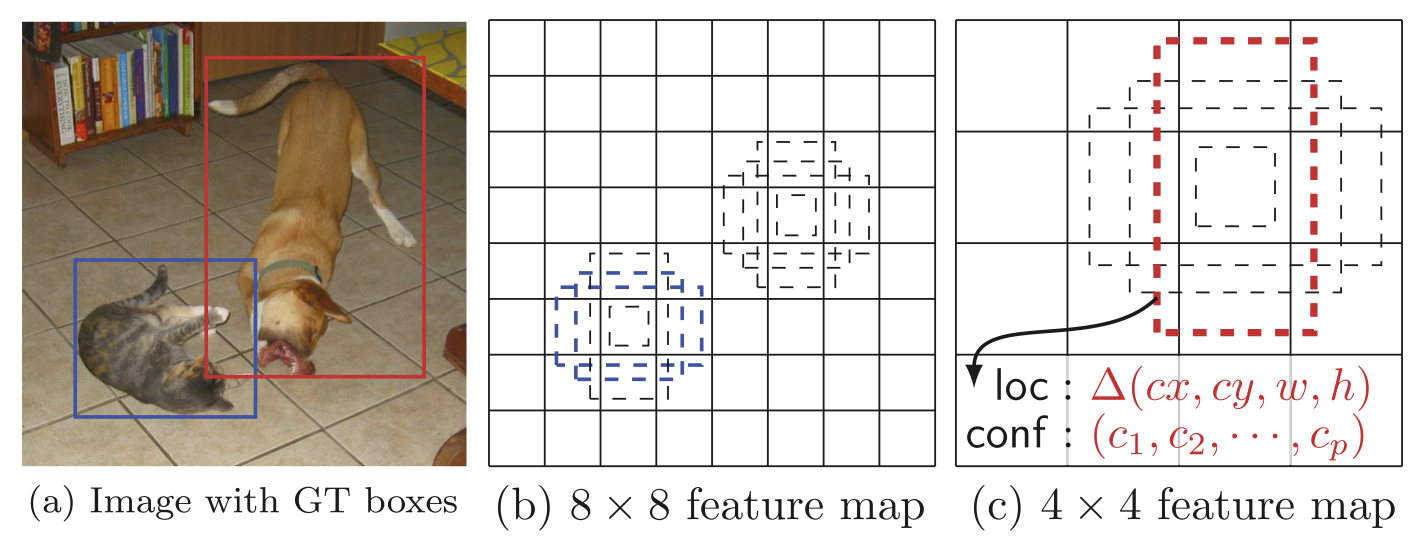
\includegraphics[width=\textwidth]{figures/ssd_feature_maps_scaling.png}
	\caption[Detecting Objects at Different Scales Through SSD's Feature Maps]{The combination of bounding boxes in varying aspect ratios and multi-scale feature maps allows the SSD to detect objects in different sizes and orientations.\\
		\tiny{Source:~\cite{detectorSSD}}}
	\label{fig:ssdFeatureMapScaling} % labels always have to be placed after the caption
\end{figure}

\subsection{Architecture}

\subsection{Latest Improvements}


\chapter{App Development}

\section{Previous State of the Application} \label{sec:previousState}

The practical part of this work was built in top of the already existing Android application TUM-Lens in its version 1.0. The app is already cable of classifying images received from the live camera stream in real-time. It can also classify images that are loaded from the disk of the Android as an alternative operational mode to the camera stream classification. Moreover, the user can choose between different TensorFlow-Slim\footnote{\url{https://github.com/google-research/tf-slim}} models to classify the images. This enables the user to do two things: she can compare the speed of similar detectors and she can also change the type of objects that can be detected as some of the available networks were trained on different data~\cite{maxJokel} and with different class labels. The most impactful design decision of the former developer of TUM-Lens was to run the entire classification locally on the Android device.

\section{Migration From Java to Kotlin}

During the Google I/O conference 2017 Google announced that they are making the programming language Kotlin a first-class citizen in Android~\cite{googleIO17}. Two years later, Google refined this statement annunciating that Android development will "be increasingly Kotlin-first" and, at the present day, the Google Developers website recommends developers to choose Kotlin when they start building a new Android app~\cite{kotlinFirst}. This alone can be reason enough to migrate an application to Kotlin - especially as long as its code base is still as manageable as the code base of TUM-Lens. To provide further explanations for the soundness of such a step we will first look at the advantages of Kotlin over Java - with particular emphasis on the context of TUM-Lens being developed by students as part of their final theses. After that, we look at the code conversion process from Java to Kotlin which is backed by powerful functionality integrated into Android Studio. We will also see an example for a pitfall that can be easily overlooked in such a semi-automated conversion process. Finally, we analyse how the number of lines of code changed from the Java files in app version 1.0 compare to their current state being fully migrated to Kotlin.

\subsection{Advantages of Kotlin}
Continuing the development of TUM-Lens in Kotlin has several advantages. As the is app currently exclusively developed by students, Kotlin's enhanced expressiveness and conciseness over Java makes it easier for fellow students to understand the entire application within the scope of a bachelor's or master's thesis. Moreover, students can learn more in the given amount of time they spend working on the app because they can focus more strongly on the implementation of new features instead of having to write boilerplate Java code. As students are more error prone than professional developers they surpassingly benefit from the safety features integrated into the Kotlin language. The most common cause for crashes of Java applications is the null pointer exception~\cite{nullPointerSamebug, nullPointerOverops}. With Kotlin being a strongly typed language a lot of these null pointer exceptions will be avoided because Kotlin's safety features help the developer to identify potential sources of such errors very easily. Google itself claims that Android apps are 20\% less likely to crash when they contain Kotlin code~\cite{kotlinFirst}.

\subsection{Converting Java Files to Kotlin Files}

Android Studio offers a convenient way to convert files from Java to Kotlin. On macOS, we first have to open the Java file we want to migrate in Android Studio. Next, we select \textit{Code} from the menu bar and then the menu item \textit{Convert Java File to Kotlin File}. If we have not yet configured Kotlin in your project, Android Studio will prompt us to ether do so or abort the migration process. Once Kotlin is set up Android Studio will immediately start the conversion. At the end of the process we are prompted with a dialogue asking "Some code in the rest of your project may require corrections after performing this conversion. Do you want to find such code and correct it too?" which we confirm by clicking on the yes-button. They file has now been converted from Java to Kotlin. In some cases the resulting Kotlin code works right away but in the context of TUM-Lens manual adjustments were mandatory in every file because of several reasons. \\

For a start, Android Studio could not always infer all types automatically. With Kotlin being strongly typed it was necessary to restructure the code so that the compiler could know each variable's type or safely cast a variable to the appropriate type (called \textit{Smart Cast} in Kotlin). We solved this situation using two different approaches distinguished by the importance of the successful execution of the respective code block. In the case of non-critical functionality, using Kotlin's safe call operator \code{?.} to access properties that might be null was sufficient. When it came to core functions, wrapping such functionality in an additional safety check was the better option. This not only capacitates the compiler to be certain that a mutable property had not accidentally become null before being accessed. It also enables us to react appropriately if the safety check fails. \\

\begin{lstlisting}[style=standard, language=Kotlin, label=code:kotlinProperty, caption={Kotlin's declaration syntax for a mutable property. Getter and setter are optional. The property type is only optional when the compiler can infer it from the context (meaning either from the initializer or from the return type of the getter).}]
var <propertyName>[: <PropertyType>] [= <property_initializer>]
	[<getter>]
	[<setter>]
\end{lstlisting}

Apart from type inference, there was one part to Android Studio's built-in code migration that actually tricked us into introducing a bug: the conversion of getters and setters. \autoref{code:kotlinProperty} shows the syntax for the declaration of a property in Kotlin. Every property has default public getters and setters if not explicitly defined otherwise. Java, on the other hand, conventionally defines methods like \code{public variableType getVariableName()} and \code{public void setVariableName(variableType newValue)} for every variable of a private class that shall be retrieved or overwritten from outside that class. \\

\autoref{code:bugSourceJava} contains the original Java code and listing \autoref{code:bugSolutionKotlin} shows the final solution that implemented in addition to Kotlin's property accessors. The default Kotlin getter is not enough here as it would omit the crucial conversion task. However, this is exactly what happened during the auto-conversion. As a result, other parts of the logic broke because the \code{rgbBytes} object could not be properly processed which lead to the application not working as expected. In this special case some accessors of the property were in need of the image conversion and others were not. Therefore, we did not put the image conversion into a custom accessor because we did not want to call \code{imageConverter!!.run()} every time the property was used. Placing it in the separate method \code{getConvertedRgbBytes()} has therefore been a good decision for us.

\begin{minipage}[t]{0.41\linewidth}
	\begin{lstlisting}[style=standard, language=Java, label=code:bugSourceJava, caption={Java code that lead to the introduction of a bug after using Android Studio's built-in Java to Kotlin converter.}]
protected int[] getRgbBytes() {
	imageConverter.run();
	return rgbBytes;
}
	\end{lstlisting}
\end{minipage}
	\hfill
\begin{minipage}[t]{0.48\linewidth}
	\begin{lstlisting}[style=standard, language=Kotlin, label=code:bugSolutionKotlin, caption={Substituting the wrongly placed default Kotlin accessors with this method solved the problem.}]
protected fun getConvertedRgbBytes(): IntArray? {
	imageConverter!!.run()
	return rgbBytes
}
	\end{lstlisting}
\end{minipage}

\subsection{Measuring The Decrease of The Size of The Code Base} %TODO: Check if this should rather be moved to the Results chapter

Using the npm distribution of the tool Count Lines of Code (cloc)\footnote{Original cloc project by Al Danial: \url{https://github.com/AlDanial/cloc}\\cloc npm distribution by Kent C. Dodds: \url{https://www.npmjs.com/package/cloc}} we can easily count lines of Java and Kotlin code while ignoring blank lines and comment lines. This enables us to monitor how the shift from Java to Kotlin influenced the number of lines of code. With Perl, Node and npm installed on our machine,
we run the following command which prints its output to stdout:

\begin{lstlisting}[style=standard, language=bash, label=code:cloc, caption={npx cloc command with its options and arguments. Prints the lines of code analysis comapring files before and after the Java to Kotlin conversion. The output was also saved as cloc.csv and can be found in lens-david/thesis/raw\_data.}]
	(base) david@DDs-MBP lens-david % npx cloc --by-file --git-diff-rel --match-d='main' --include-lang=Java,Kotlin -csv f6a18e0f 031a26a7
\end{lstlisting}

The \code{--by-file} option enables us to directly compare each Java file with Kotlin equivalent as it changes the output so that the results are returned for every source file encountered. \code{--git-diff-rel} interprets the command line arguments as git targets and compares only files which have changed in either commit which is exactly what we need to measure the change in the number of lines of code. Only files in the main directory are of our concern so we let cloc only search this directory using the option \code{--match-d='main'}. This excludes e.g. the test directory from being searched. With \code{--include-lang=Java,Kotlin} we limit the output to files written in the languages we seek to collate. Other files like Android's XML layout files are not of interest for this analysis. Finally, we provide two git commits. \code{f6a18e0f} is the last commit pushed by the previous developer of TUM-Lens and \code{bf0dbf7f} is the more recent commit that does not contain Java files anymore but replaced them with their respective Kotlin substitute.

\begin{table}[h]
	\begin{tabularx}{\columnwidth}
		{ >{\RaggedRight}p{10cm} | C }
		\hline
		Files in TUM-Lens v1.0 migrated from Java to Kotlin	&	Delta in lines of code	\\	\hline \hline
		CameraRoll	&	-34	\\	\hline
		Classifier	&	4	\\	\hline
		ListSingleton	&	-9	\\	\hline
		PermissionDenied	&	-8	\\	\hline
		StartScreen	&	-12	\\	\hline
		ViewFinder	&	-7	\\	\hline
		fragments/CameraRollPredictionsFragment	&	9	\\	\hline
		fragments/CameraSettingsFragment	&	-15	\\	\hline
		fragments/ModelSelectorFragment	&	5	\\	\hline
		fragments/PredictionsFragment	&	4	\\	\hline
		fragments/ProcessingUnitSelectorFragment	&	-7	\\	\hline
		fragments/SmoothedPredictionsFragment	&	6	\\	\hline
		fragments/ThreadNumberFragment	&	-6	\\	\hline
		helpers/App	&	1	\\	\hline
		helpers/CameraEvents	&	0	\\	\hline
		helpers/FreezeAnalyzer	&	-6	\\	\hline
		helpers/FreezeCallback	&	0	\\	\hline
		helpers/ImageUtils	&	43	\\	\hline
		helpers/Logger	&	6	\\	\hline
		helpers/ModelConfig	&	-2	\\	\hline
		helpers/ProcessingUnit	&	-2	\\	\hline
		helpers/Recognition	&	-26	\\	\hline
		helpers/ResultItem	&	-21	\\	\hline
		helpers/ResultItemComparator	&	-2	\\	\hline \hline
		\fontseries{b}\selectfont{cumulative delta over all relevant files}	&	\fontseries{b}\selectfont{-79}	\\ \hline
		\end{tabularx}
	\caption[Java Files in TUM-Lens v1.0 And Change in Lines of Code After Their Conversion to Kotlin]{This table shows the results from the command line prompt in \autoref{code:cloc}. Packages have been indicated as a prefix to the file name to resemble the original project structure of TUM-Lens v1.0 and file extension have been omitted. Overall, the total size of the codebase shrank because of the migration from Java to Kotlin. This is particularly impressive as understandably further logic was added to existing classes in order to account for the new object detection functionality.}
	\label{tab:cloc}
\end{table}


\section{Implementing Object Detection Using The TensorFlow Lite Framework}

As described in \autoref{sec:previousState} the core feature of TUM-Lens v1.0 is image classification. Most notably, the classification task is not outsourced to some remote server but performed offline on the device itself. We adhere to this decision and built our logic on top of Google's TensorFlow Lite example app for object detection~\cite{tfSampleAppGuide, tfSampleAppRepo}. The detection task is therefore carried out locally using the same TensorFlow-Lite API as the image classification. We also integrate our detection results into the images received from the camera live-stream so that the user of the app can experience the object detection in real-time. This being said, there is some discrepancy to the existing set of functionalities built around the image classification. Only one model for object detection is currently available within the app and the detection logic cannot be applied to images that have been loaded from the storage of the device.


\subsection{Expansion of The Existing App Architecture}

In order to make the structure of the app more accessible to new developers we put the core classes responsible for image classification and object detection into two distinct packages. The project now includes the four packages \code{classification}, \code{detection}, \code{fragments} and \code{helpers}. Only the two base activities \code{StartScreenActivity} and \code{PermissionDeniedActivity} remained on the top-level.

\begin{figure}[H] % [H] for HERE
	\centering
	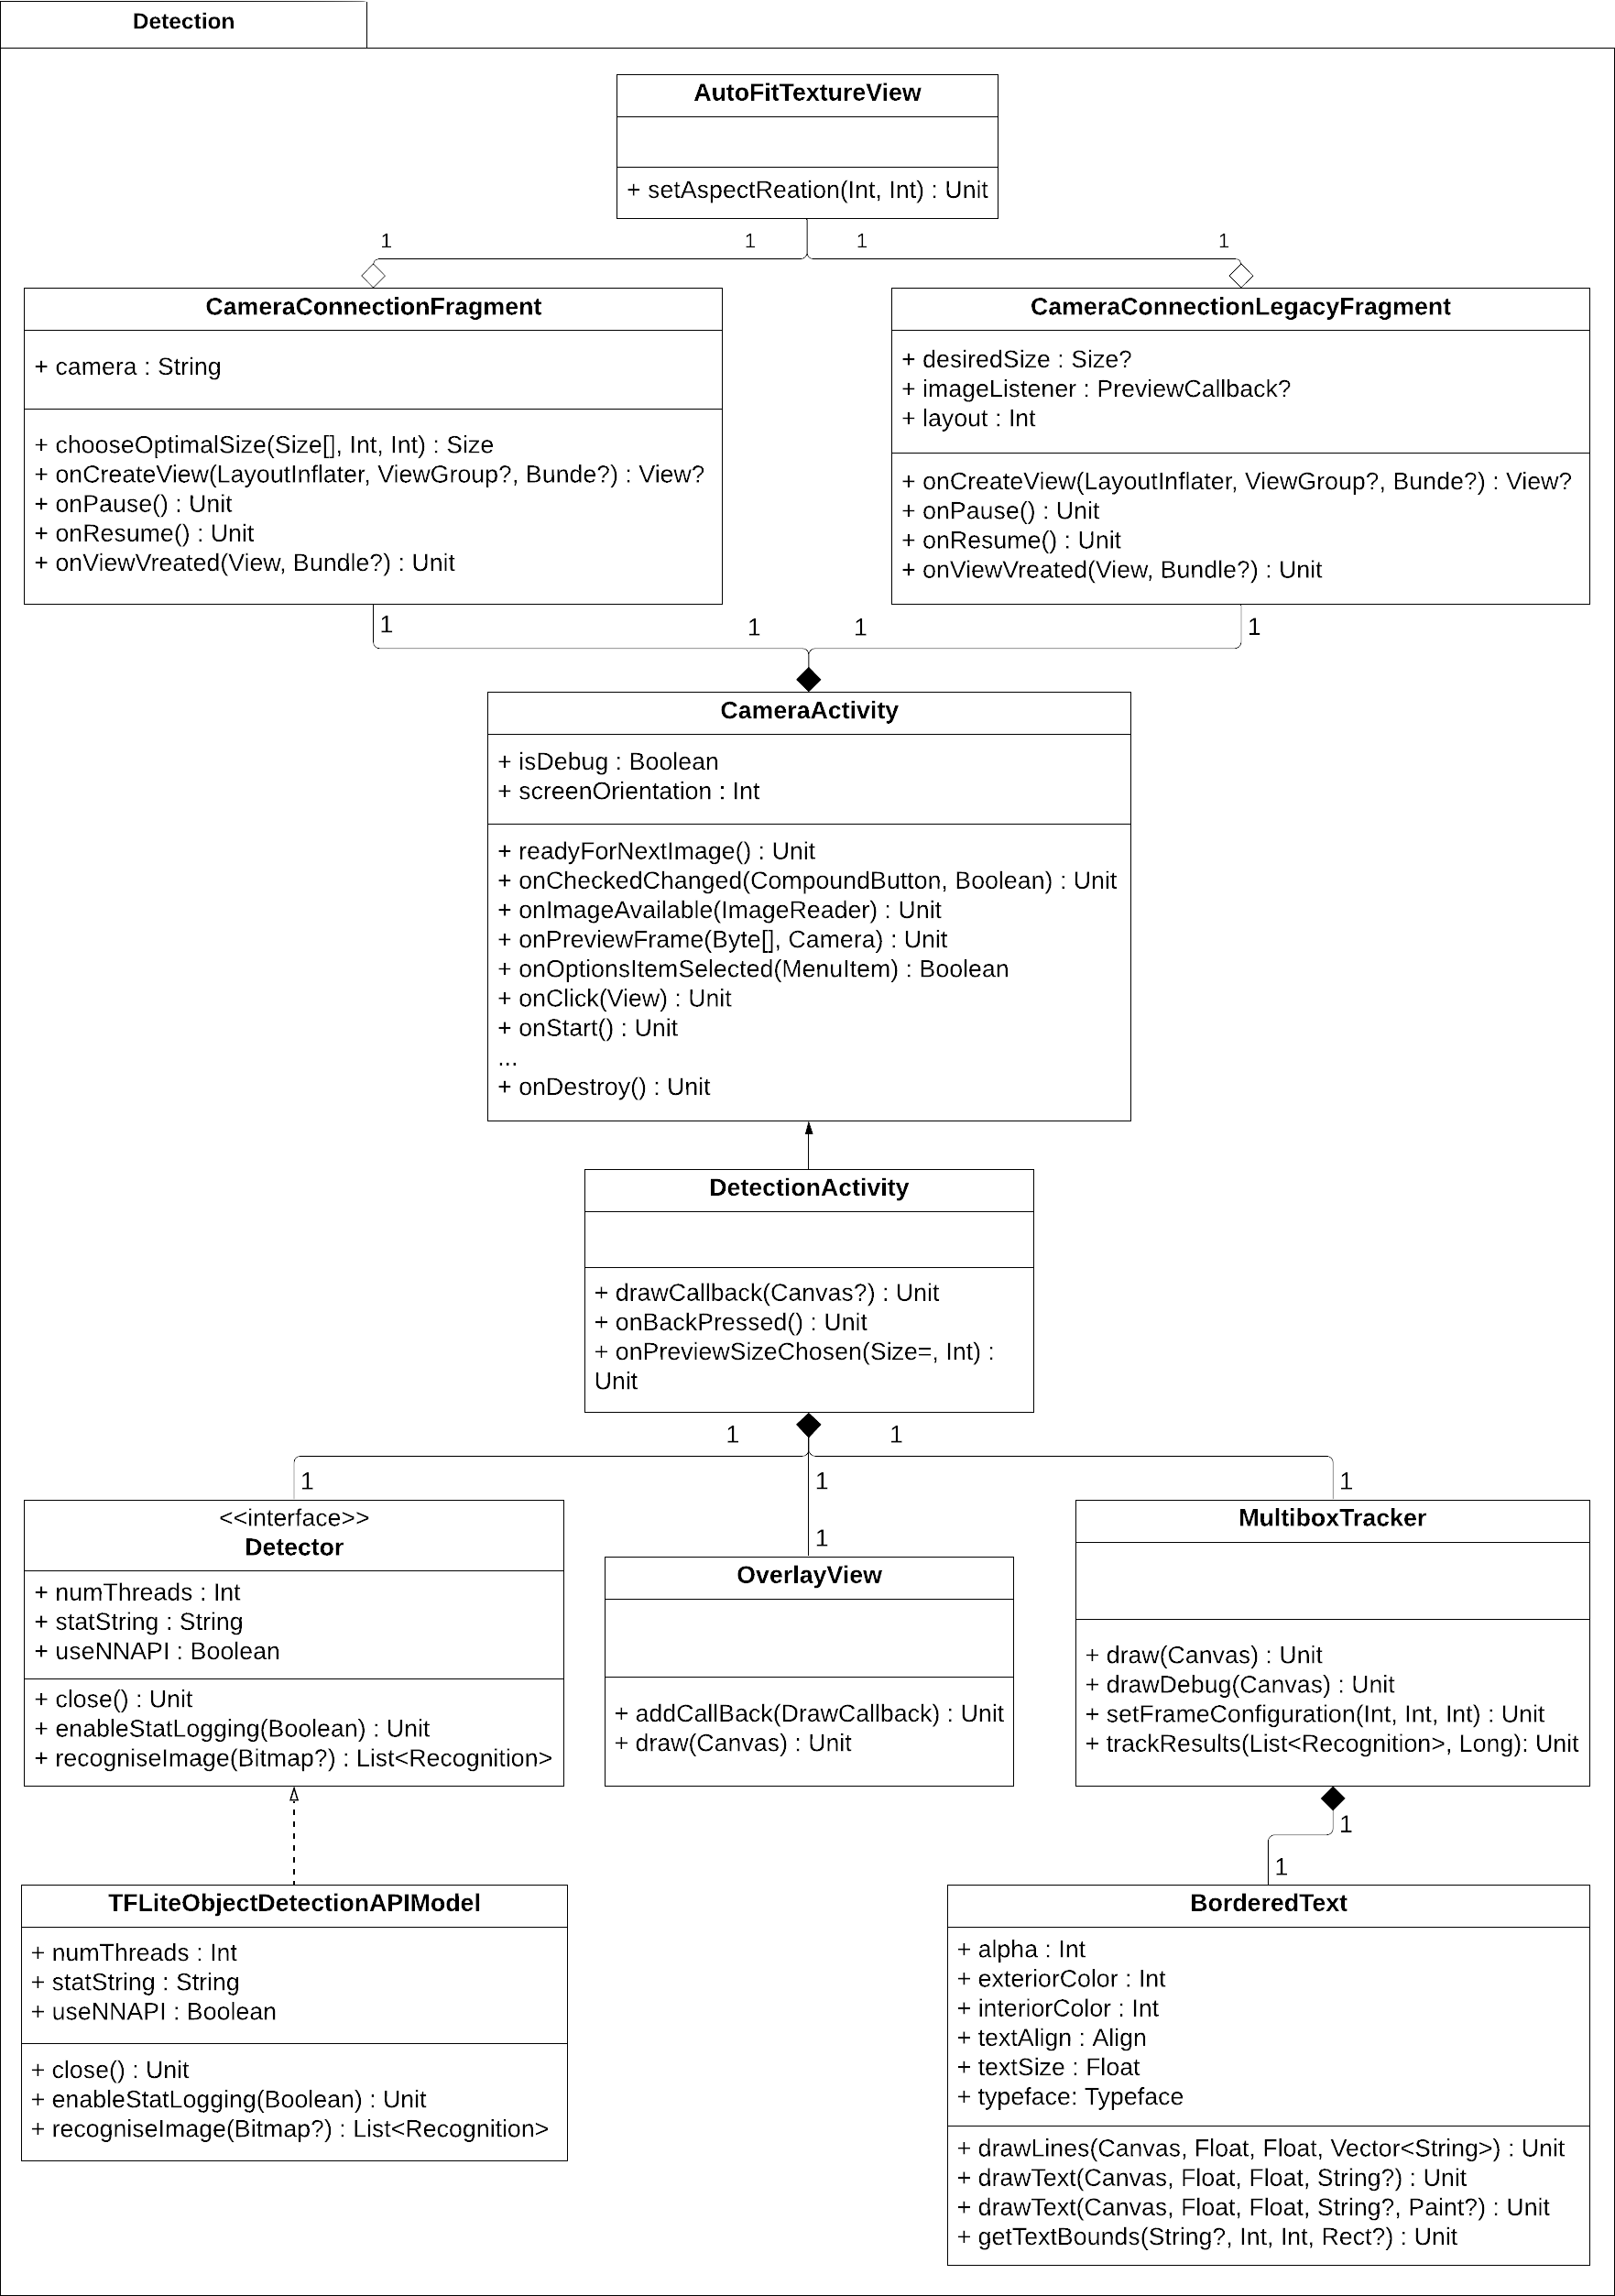
\includegraphics[width=\textwidth]{figures/uml_detection_package.png}
	\caption[UML Class Diagram of The New Detection Package]{UML class diagram of the new detection package. Only public properties and methods are shown.}
	\label{fig:umlDetectionPackage} % labels always have to be placed after the caption
\end{figure}


\subsection{DetectionActivity}

Just as \code{ClassificationActivity} is the core activity that handles the image classification of the camera feed, the new \code{DetectionActivity} is the central activity for object detection. The user can easily switch between the different mode of image analysis by using a toggle button on top of the screen. We decided to use a toggle switch here since there are exactly two operating modes (classification and detection) and they are working mutually exclusive in order to best utilise the computation power of the device. This design decision may be revised later when the scope of the app is expanded to cover more visual tasks (see \autoref{sec:cvtasks} for examples of such tasks). Another reason for a rework can be the fact that mobile devices might have enough computing power so that solving multiple tasks in parallel does not make a noticeable difference for the app user, meaning images are still processed in real-time.

\subsubsection{Inheritance}

\code{DetectionActivity} inherits from the abstract class \code{CameraActivity} and implements the \code{OverlayView.DrawCallback} interface. The \code{CameraActivity} handles all communication with Androids camera API and implements the proper setup and behaviour of the elements in the bottom sheet. The \code{DrawCallback} provides a single function definition that the \code{DetectionAcitivty} overrides in order to render the detected objects as rectangles in a layer on top of the preview of the camera image stream.

\subsubsection{Bitmap Conversion}

Since TUM-Lens can run on a multitude of devices with varying combinations of camera and display resolution, the \code{DetectionActivity} sets parameters such as font sizes and matrices to convert the image data back and forth between the different formats the data is needed in. This is important as in contemporary Android devices, the resolution of the camera is usually above the resolution of the display. This is also the case for the Xiaomi Mi 9 on which we tested the application during its development (see \autoref{chap:specs} for its technical specifications). Sticking to the example of Xiaomi Mi 9, the images captured by the camera have 20 (selfie camera) or 45 (main camera) megapixels and are scaled down to 2.5 megapixel to be displayed on the device screen. After that, they are again scaled down to a bitmap of 300x300 pixels\footnote{The image received by the detector might indeed be even smaller than 300x300 pixels as the camera input is usually not square and the aspect ratio is kept throughout the image conversion pipeline. Therefore, the 300 pixels denote the larger dimension (width or height) of the input bitmap.} as this is the appropriate input size for the implemented detection framework described in \autoref{sec:mobilessd}. Once the detector returns bounding boxes for the objects detected in its input image the coordinates of these rectangles in turn are scaled back up to mark the corresponding areas in the higher resolution image shown on the device display.

\subsubsection{Detection and Tracking}

The \code{DetectionActivity} also orchestrates the two most fundamental tasks of the object detection process: object detection and, since the images are derived from a continuos camera stream, object tracking. It instantiates the object \code{detector} of the class \code{TFLiteObjectDetectionAPIModel} to handle the interactions with the TensorFlow Lite \gls{api} and a \code{MultiBoxTracker} object \code{tracker} that tries to assign each rectangle drawn on the screen to its related recognition result across successive input images. This is important because the bounding boxes that are drawn as an overlay on the camera view use different colours for different objects. If no tracking would happen, the colour that is assigned to an object will change randomly with every new image the detector processes. This would be very confusing for the user. Therefore, the recognition results returned by the detector are not directly rendered on the screen but first processed by the \code{tracker}. \\

The \code{tracker} guarantees two properties: Firstly, empty or degenerated recognition results are skipped and not tried to be displayed. Secondly, the 15 colours the \code{tracker} can assign to the remaining objects are  allocated in the same order every time the old drawings are cleared from the canvas and new ones are drawn. This process of detecting objects, clearing old rectangles from the screen and drawing new ones happens with every image the detector processes. While the tracking is far from perfect, the order in which recognitions are returned by the detector stays roughly the same. This happens because they are ordered by the coordinates of their bounding boxes. Depending on the camera settings, the camera can usually stream 30 to 60 frames per second. If the user doesn't move the camera surpassingly fast, the coordinates of the recognition results stay close enough together so that they get assigned the same colour across the changing camera images. New  objects appearing in the scene (or existing ones becoming larger as the user gets closer) are currently the major cause for inconsistent object colouring. However, as long as no new objects are recognised, the existing ones tend to keep their colours. This is already a great achievement given the tracking is purely based on properties of the TensorFlow Lite \gls{api} and does therefore add effectively non-existent overhead to the object detection pipeline. \\

The detection threshold is set to 0.5 in order to display the most relevant objects. Hence, only recognition results received from the \code{detector} that have a confidence score of 0.5 or higher are handed to the \code{tracker}. This further improves the user experience supplementary to the object tracking.


\subsection{Dive Into}
\subsection{Object Detection}
\subsection{Implementation Fun}

\subsection{Next steps in the development of TUM-Lens}

% Potential Contets: Design and architecture choices, reused patterns from exisiting application, improvements to exisiting code
% Add model selector for different detectors as well

\chapter{Results}

Kotlin made the code definitely more concise

\section{Performance Evaluation}

\section{Accuracy}

\section{Possible Applications} % Can also be named "Future Work" depending on the contents of this section

Die Anwendungsbereiche von Computer Vision sind zahlreich. Zu den regelmäßigen Aufgaben im Bereich 

Organisation von Fotos auf dem Smartphone, ohne dass diese an die Server von Apple, \& Google Co geschickt werden müssen (Gruppieren von Fotos, die zu einem Urlaub gehören, Gesichtserkennung, Objekterkennung)

Autonome Autos werden unahängig von einer Verbindung zum Internet (5G, shared medium, bleibt das Auto im Tunnel dann stehen?)

\section{Future Work}

Replace depracted functionalities

Add more models to chose from for object detection

Apple object detection to files loaded from storage

Change the apps infrastructure so that models (don't forget the labels though) can be loaded from a server (suitable as they tend to be rather small). This would make it easier to add new models on the fly.

Use real tracking to track objects across consecutive input images 
% -------------------------------------------------------------------------------
% ----------------------------------- APPENDIX --------------------------------
% -------------------------------------------------------------------------------

\appendix

\chapter{Screenshots of the Application}

Compare old and new

\chapter{Test Device Specifications} \label{chap:specs}

The development of TUM-Lens v2.0 was tested on a Xiaomi Mi 9. Development and testing occurred April to August 2021. The most relevant specifications are as follows. 

\begin{table}[h]
	\begin{tabularx}{\columnwidth}
		{ >{\RaggedRight}p{4cm} | L }
		\hline
		Brand and name	&	Xiaomi Mi 9	\\	\hline
		CPU	&	Octa-core: 8 Kryo 485 cores with respective clock speeds of 1x2.84 GHz, 3x2.42 GHz and 4x1.78 GHz	\\	\hline
		GPU	&	Adreno 640	\\	\hline
		RAM	&	6.00 GB	\\	\hline
		Screen resolution	&	1080 x 2340 pixels ($\approx$ 2.5 MP)	\\	\hline
		Screen aspect ratio	&	19.5:9 \\ \hline
		Screen size (diagonal)	&	6.39 inches	\\	\hline
		Main camera (triple)	&	48 MP, f/1.8, 27mm (wide), 1/2.0", 0.8µm, PDAF \newline 12 MP, f/2.2, 54mm (telephoto), 1/3.6", 1.0µm, PDAF \newline 16 MP, f/2.2, 13mm (ultrawide), 1/3.0", 1.0µm, PDAF	\\	\hline
		Selfie camera (single)	& 20 MP, f/2.0, (wide), 1/3", 0.9µm \\ \hline
		Model identifier	&	M1902F1G	\\	\hline
		MIUI version	&	MIUI Global 12.0.5 (QFAEUXM)	\\	\hline
		Android version	&	10 QKQ1.190825.002	\\	\hline
		Release Date	&	25th of March 2019	\\	\hline
	\end{tabularx}
	\caption[Test Device Specifications]{Test Device Specifications}
	\label{tab:specs}
\end{table}




\chapter{Tips With Greetings From the Chair}
\label{sec:tips}       % labels can be put almost anywhere and can be referencef from anywhere.
Here are tips along the way:

\section{Tips}
\subsection{How to Describe}
% optional: set the spacing between columns
\setlength{\columnsep}{30 pt}
When listing several points you have three basic options:
\begin{multicols}{3}
	\begin{itemize}
		\item itemize
		\item enumerate
		\item description
	\end{itemize}
	
	\vfill\null
	\columnbreak
	
	\begin{enumerate}
		\item itemize
		\item enumerate
		\item description
	\end{enumerate}
	
	\vfill\null
	\columnbreak
	
	\begin{description}
		\item[itemize] short, unordered
		\item[enumerate] short ordered
		\item[description] listing of descriptions. Also nice for longer ones.
	\end{description}
	
\end{multicols}


\subsection{How to Quote}

\begin{quote}
	"This is a quote!"
\end{quote}

\begin{itemize}
	\item Citations to a source can be made like this \verb|\cite{gratl17task}| =~\cite{gratl17task}
	\subitem Always join text and the citation with a non-breaking space: \verb|text~\cite{foo}|.
	\item Referencing Sections, Figures, Tables, Formulas: \verb|\autoref{sec:tips}| = \autoref{sec:tips}.
	\item Footnotes for url or further notes: \verb|\footnote{\url{https://www.top500.org}}| = \footnote{\url{https://www.top500.org}}
\end{itemize}

\subsection{How to Math}

Use the align environment for equations especially if you want to align them somehow.

\begin{align}
	1 + 1 &\ne 3\\
	\left(\dfrac{10}{1}\right) - 9 &= 1
\end{align}

% if you need a pagebreak because figure placement is broken:
\clearpage

\section{Environments}

\subsection{How to Figure}

Anything can also be put in multiple columns.

\begin{multicols}{2} % defines an environment with two columns
	\begin{figure}[H] % [H] for HERE
		\centering
		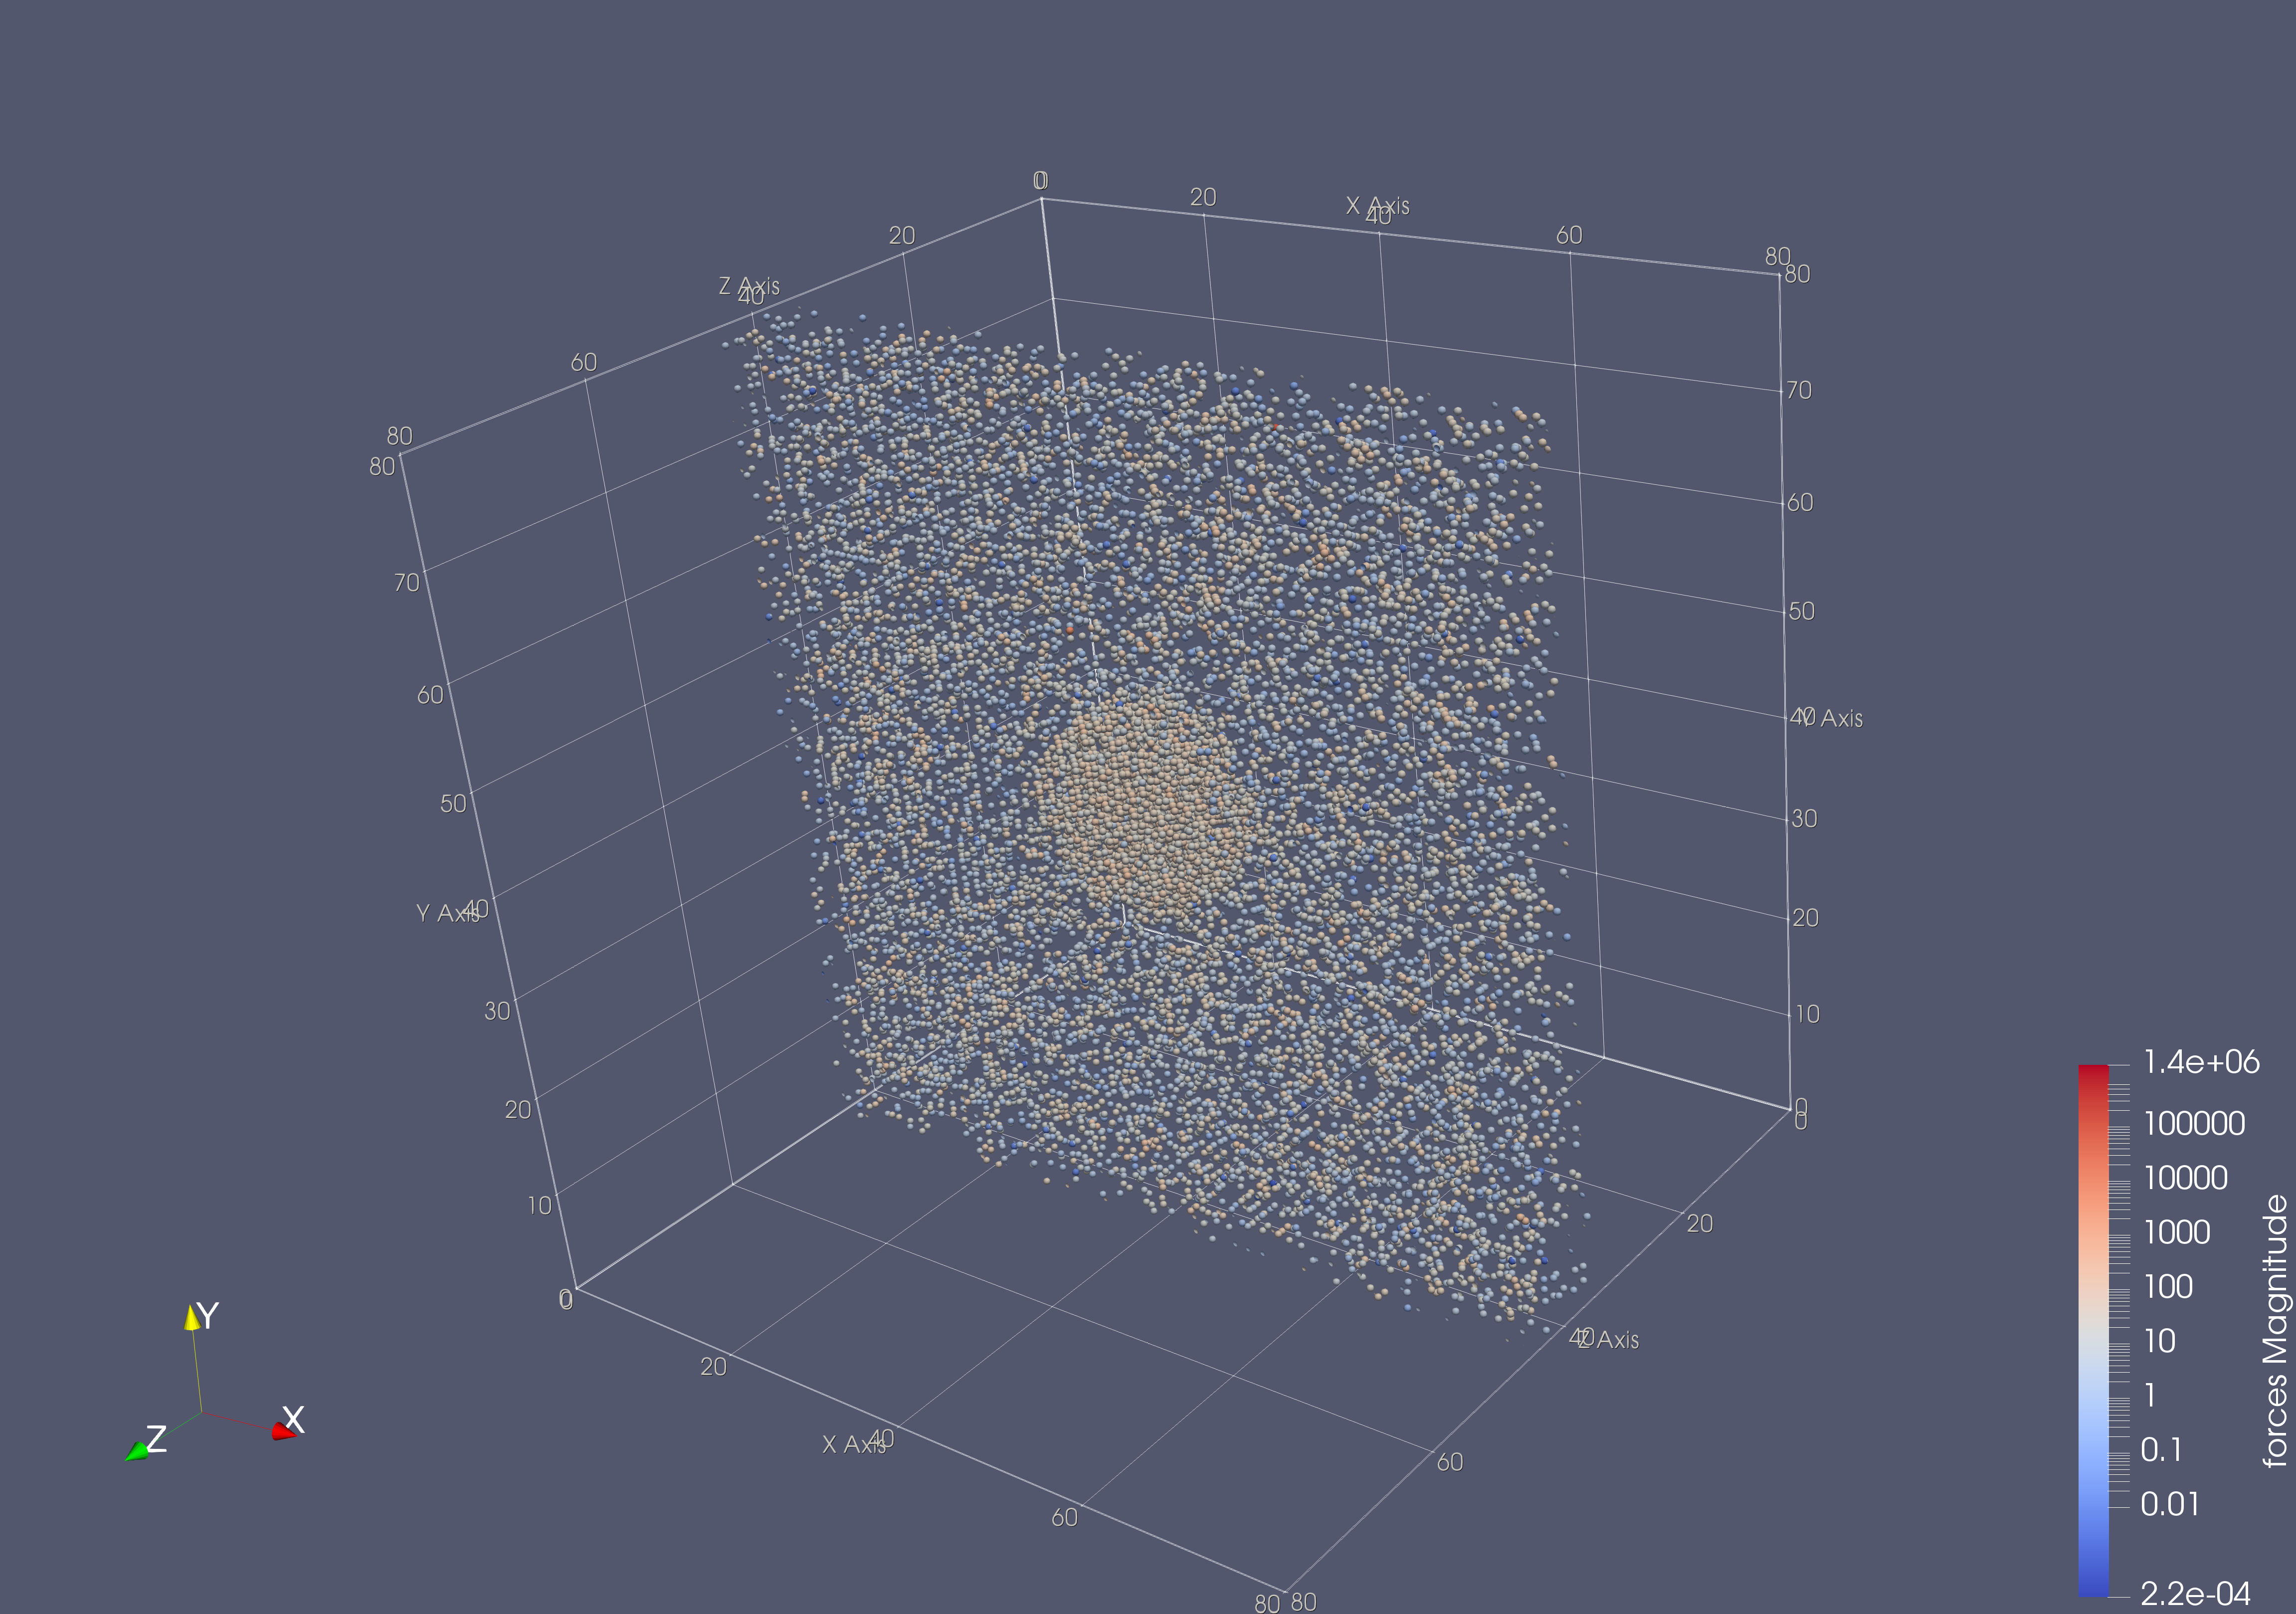
\includegraphics[width=.9\columnwidth]{figures/scenario_clip_rot.png}
		\caption[Example Figure]{Some Caption. Always also include a source if it wasn't created by you!\\
			\tiny{Source:~\cite{gratl17task}}}
		\label{fig:exampleLabel1} % labels always have to be placed after the caption
	\end{figure}
	
	\columnbreak    % start next column
	
	\begin{figure}[H]
		\centering
		\begin{tikzpicture}
			\node[anchor=south west,inner sep=0] (image) at (0,0) {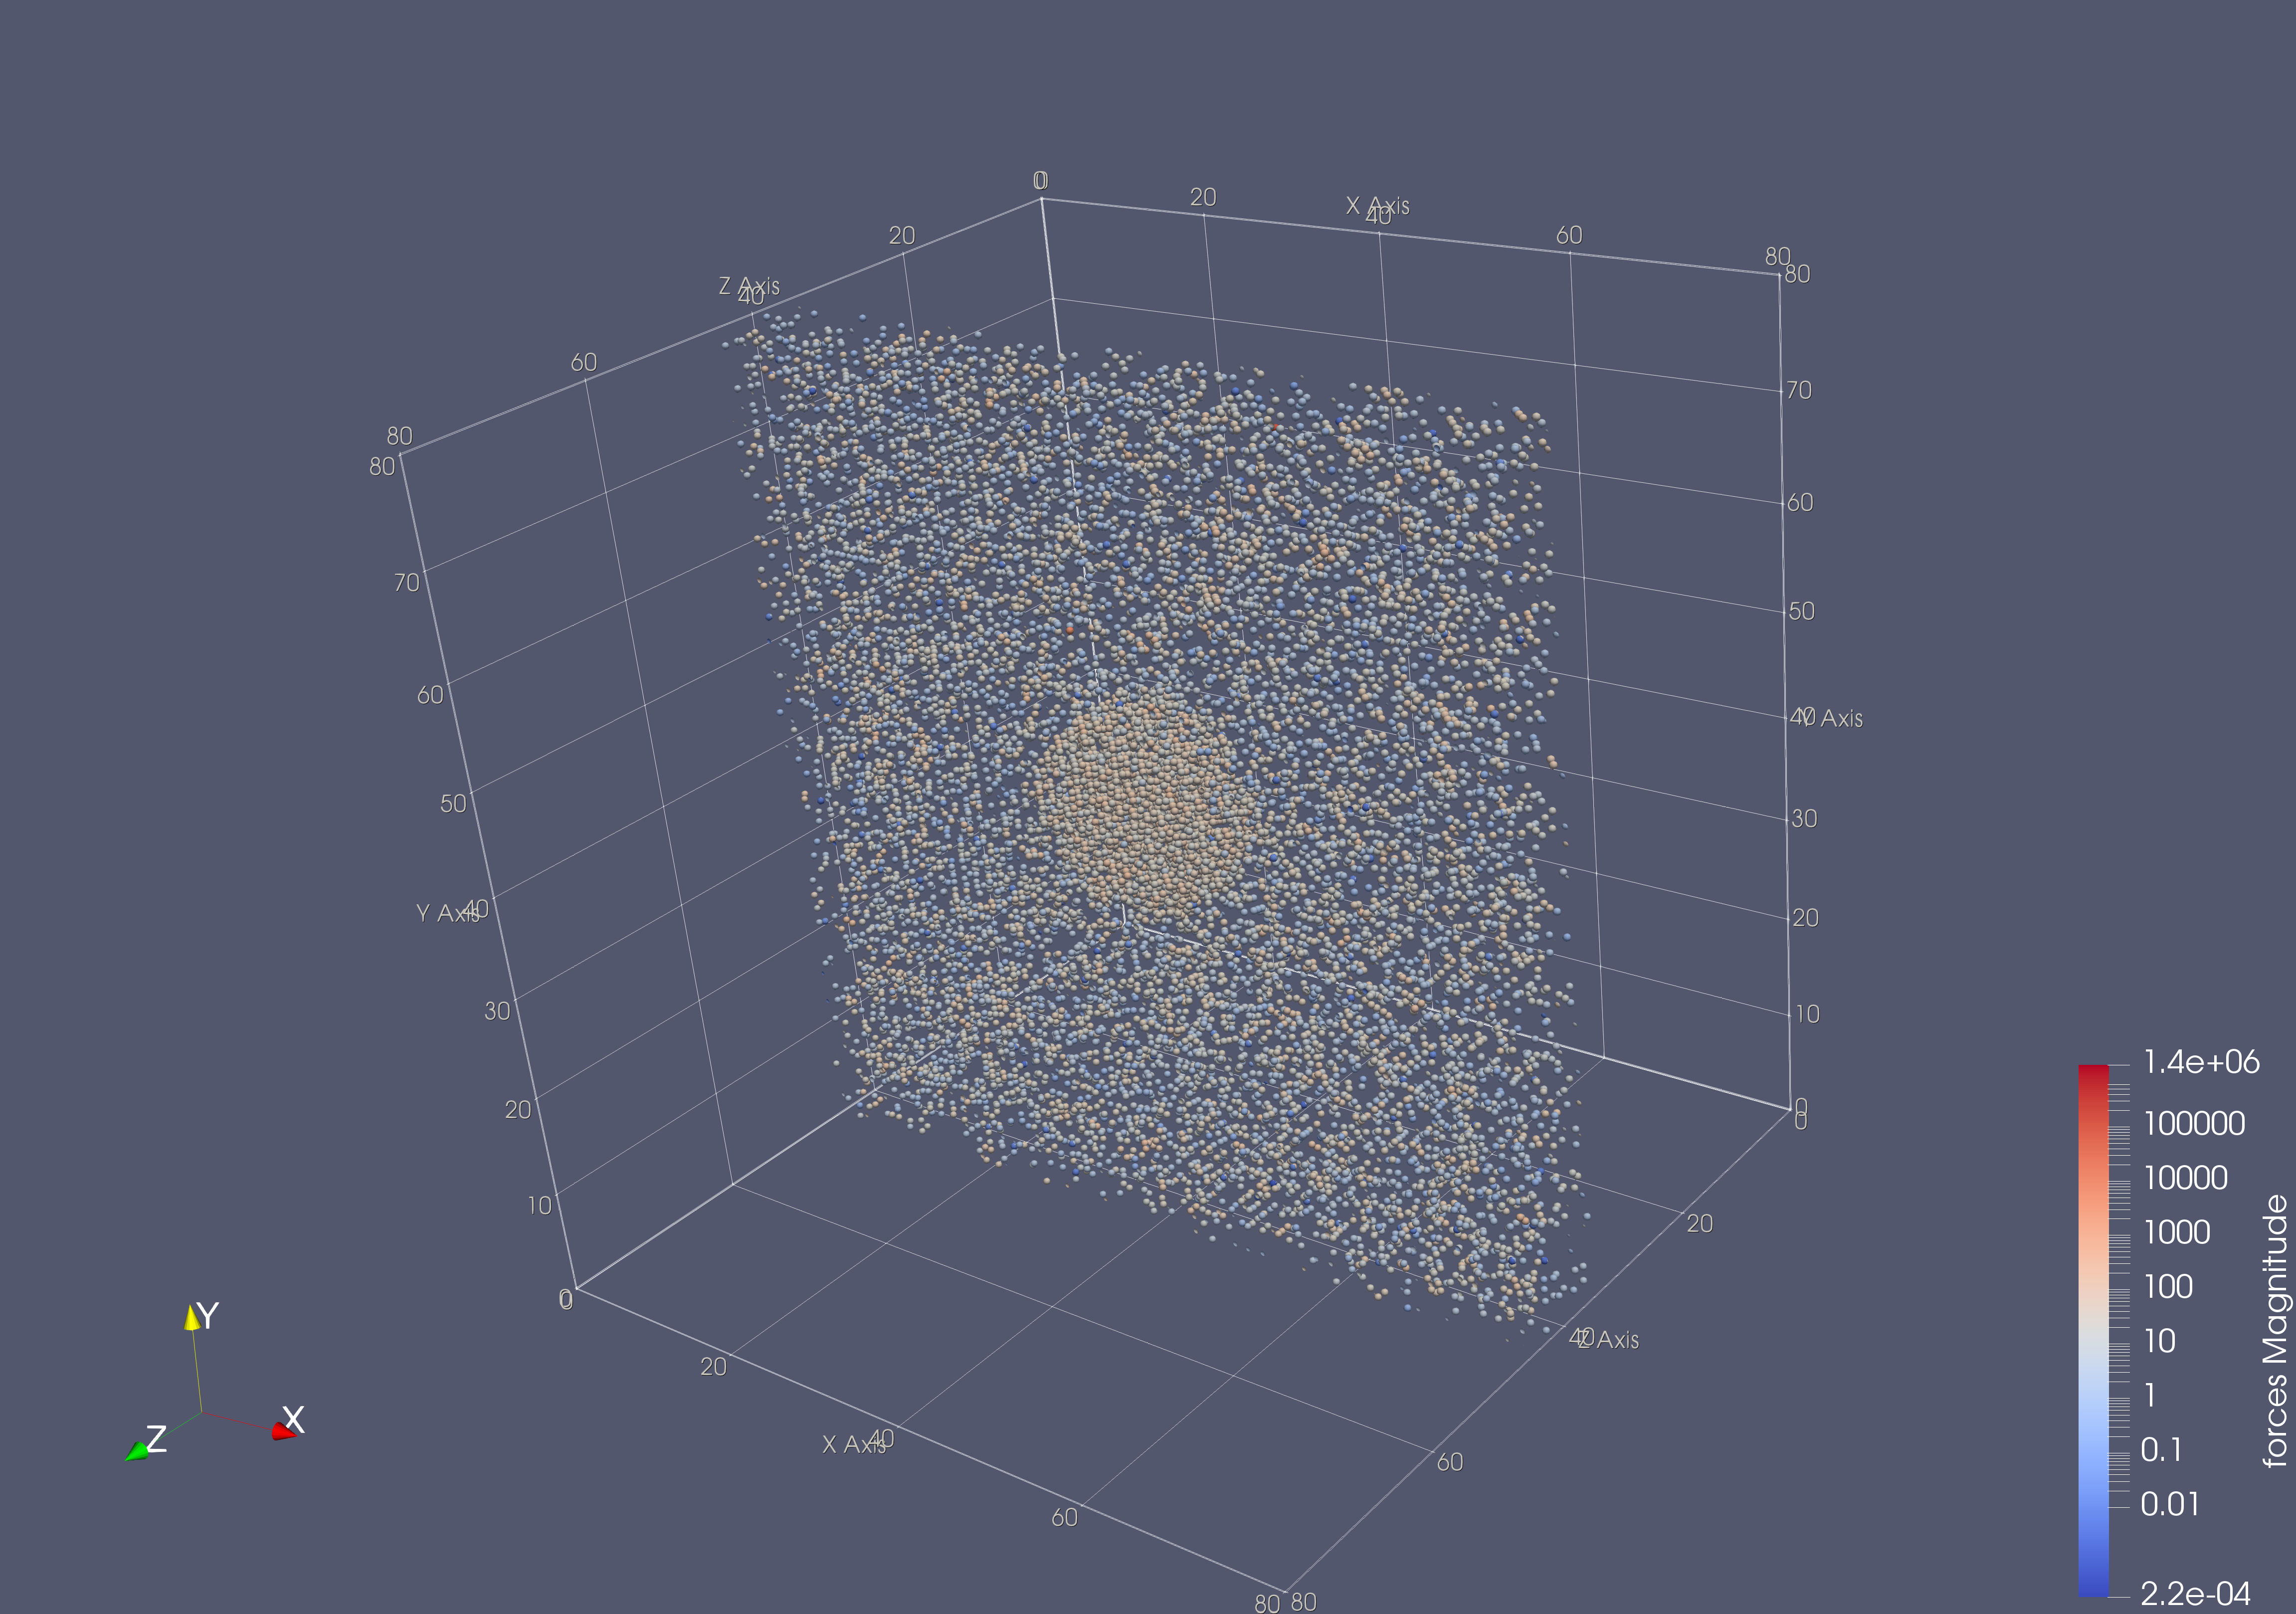
\includegraphics[width=.9\columnwidth]{figures/scenario_clip_rot.png}};
			\begin{scope}[x={(image.south east)},y={(image.north west)}]
				\draw[red, thin,rounded corners] (.42,.42) rectangle (.58,.6);
			\end{scope}
		\end{tikzpicture}
		\caption[Figure with tikz]{Figures can be drawn on or completely generated with tikz.}
		\label{fig:exampleLabel2}
	\end{figure}
\end{multicols}

\paragraph{Subfigures}
If grouping of several pictures seems reasonable, think about using subfigures. This often comes in handy with plots.

\begin{figure}[H]
	\centering
	\begin{subfigure}[b]{0.33\textwidth}
		\includegraphics[width=\textwidth]{example-image-a}
		\caption{example-image-a}
		\label{fig:example-image-a}
	\end{subfigure}
	\begin{subfigure}[b]{0.33\textwidth}
		\includegraphics[width=\textwidth]{example-image-b}
		\caption{example-image-b}
		\label{fig:example-image-b}
	\end{subfigure}
	\begin{subfigure}[b]{0.33\textwidth}
		\includegraphics[width=\textwidth]{example-image-c}
		\caption{example-image-c}
		\label{fig:example-image-c}
	\end{subfigure}
	\caption{One caption to describe them all.}
\end{figure}

\subsection{How to Algorithm}

\begin{figure}
	\begin{algorithm}[H]
		
		% Define custom keywords
		\SetKwFunction{KwNot}{not}
		% Define custom Functions
		\SetKwFunction{Fissorted}{is\_sorted}
		\SetKwFunction{Fbogosort}{bogosort}
		\SetKwFunction{Fshuffle}{shuffle}
		\SetKwProg{Fn}{Function}{:}{}
		\KwIn{\tabto{2cm}data array}
		\KwOut{\tabto{2cm} data sorted}
		\BlankLine
		
		\tcp{Checks if array is sorted}
		\Fn{\Fissorted{data}}{
			\For{i $\leftarrow$ 0 \KwTo data.size() - 1}{
				\label{algo:for}            % labels can also be put in the algorithm
				\If{data[i] $>$ data[i+1]}{
					\Return false
				}
			}
			\Return true
		}
		
		\tcp{actual algorithm}
		\Fn{\Fbogosort{data}}{
			\While{\KwNot \Fissorted{data}}{
				random.\Fshuffle{data}
			}
		}
		
		\caption[Bogosort]{Bogosort}
		\label{algo:example}
	\end{algorithm}
	\caption{some description what is happening}
\end{figure}

\clearpage

\subsection{How to Code}
\begin{lstlisting}[style=eclipse-cpp, caption=General form of a typical runner() function., label=code:runner]
	void runner(int type, void *data){
		switch(type)
		case taskType1:
		// do stuff using data
		case taskType2:
		// do other stuff using data
	}
\end{lstlisting}

\subsection{How to Table}
\begin{table}[H]
	\begin{tabularx}{\columnwidth}{L | C | R}
		\hline
		\hline
		bla left & bla centered\newline over two lines &  bla right\\
		\hline
		bla left & bla centered & \multirow[c]{2}{\hsize}{cell spanning two rows} \\
		\cline{1-2}
		\multicolumn{2}{c|}{cell spanning two columns} & \\
	\end{tabularx}
	\caption[Some Table]{Fancy table that can contain line breaks and extended cells.}
	\label{tab:example}
\end{table}

%TODO: Insert screenshots. Potentially even with the respective old version of a screen to see the development.

\listoffigures

\listoftables

\printbibliography

\printglossary[type=acronym,nonumberlist]

\printglossary[type=main,nonumberlist]

\end{document}
